\documentclass[10pt,spanish,mexico]{article}
\usepackage[utf8]{inputenc}
\PassOptionsToPackage{hyphens}{url}\usepackage{hyperref}
\usepackage[top = 1cm, bottom = 0.4cm, left = 0.5cm, right = 0.5cm]{geometry}
\usepackage[spanish, es-tabla]{babel}
\usepackage[table,xcdraw]{xcolor}
\usepackage[italicdiff]{physics}
\usepackage{textcomp}
\usepackage{amsthm, amssymb, amsmath, amsfonts, bbm, mathtools}
\usepackage{enumerate}
\usepackage[shortlabels]{enumitem}
\usepackage{titling}
\usepackage{wasysym}
\usepackage{lmodern} %optimiza algunas fuentes
\usepackage{float}
\usepackage{mathrsfs}
\usepackage{dsfont}
\usepackage{caption}
\decimalpoint
\usepackage{graphicx}
\renewcommand{\baselinestretch}{1}

\usepackage{multicol}
\usepackage[skip=0pt]{parskip}
\usepackage{fancyhdr}
\usepackage{titlesec}

\newcommand{\Pa}[1]{\left( #1 \right)}
\newcommand{\PA}[1]{\big( #1 \big)}

\usepackage{minted}
\setminted[cpp]{
    %linenos=false,
    breaklines=true
    %frame=leftline,
}

%Images path
\graphicspath{{img/}}

% Figuras numeradas
\usepackage{chngcntr}
\counterwithin{figure}{section}

% Ecuaciones numeradas
\numberwithin{equation}{section}

\allowdisplaybreaks

% Definiciones de mate %
\renewcommand{\theenumi}{\alph{enumi}}
\renewcommand{\labelenumi}{{\theenumi})}
\renewcommand\qedsymbol{$\blacksquare$}
\newcommand{\N}{\mathbb{N}}
\newcommand{\Z}{\mathbb{Z}}
\newcommand{\R}{\mathbb{R}}
\newcommand{\I}{\mathbb{I}}
\newcommand{\Q}{\mathbb{Q}}
\newcommand{\Zm}[1]{\mathbb{Z}/ #1 \mathbb{Z}}
\newcommand\scalemath[2]{\scalebox{#1}{\mbox{\ensuremath{\displaystyle #2}}}}

% Comandos especiales de mate
\newcommand{\pa}[1]{\left( #1 \right)}
\newcommand{\br}[1]{\left[ #1 \right]}
\DeclarePairedDelimiter{\set}{\{}{\}}
\DeclarePairedDelimiter{\floor}\lfloor\rfloor
\DeclarePairedDelimiter{\ceil}\lceil\rceil
\DeclarePairedDelimiter{\spn}{\langle}{\rangle}
\DeclareMathOperator{\sgn}{sgn}
\DeclareMathOperator{\ord}{ord}
\newenvironment{solution}
{\renewcommand\qedsymbol{$\square$}\begin{proof}[Solución]}
{\end{proof}}

\usepackage{csquotes}

\title{Referencia - ICPC}
\author{Mathgic}
\date{Junio 2025}

% Espaciado
\setlength{\columnseprule}{1pt}
\setlength{\parindent}{0pt}

\titlespacing\section{0pt}{0pt}{0pt}
\titlespacing\subsection{0pt}{0pt}{0pt}

% Header
\pagestyle{fancy}
\headheight 25pt
\fancyhead{}
\fancyfoot{}
\rhead{\thepage}
\renewcommand{\headrulewidth}{0pt}
\fancyheadoffset{0pt}
\fancyfootoffset{0pt}
\setlength\headsep{5pt}

\begin{document}


\maketitle

\begin{center}
    \href{https://github.com/SJMA11723/Data-structures-and-algorithms}{Github}
    \\ACTUALIZADO HASTA LA SECCIÓN 11. Falta 11.2.1, 11.2.2, 12, 13, etc.
\end{center}

\newpage
\tableofcontents

\newpage
\pagenumbering{arabic}
%\setcounter{page}{1}

\begin{multicols}{2}

\subsection{OJO}
\begin{enumerate}[1.]
    \item Se usan macros (MAXN, LOGN, etc) con arreglos estáticos para más comodidad, pero puede causar RTE o MLE cuando los valores son grandes. Pensar en usar \mintinline{cpp}{vector<>} (STL) cuando sea conveniente.
    %\item Temario (no oficial): \href{https://youkn0wwho.academy/topic-list}{Topic list}.
    %\item agréguenle errores/consejos que hay que tener en cuenta sobre las implementaciones y no estemos mucho tiempo tratando de encontrar el error.
\end{enumerate}

\hrulefill
\section{Templates y Testing}
\subsection{Template y archivos}
Crear una carpeta donde se estará usando la terminal y copiar lo siguiente en template.cpp
 \begin{minted}{cpp}
#include<bits/stdc++.h>
#include <ext/pb_ds/assoc_container.hpp>
#include <ext/pb_ds/tree_policy.hpp>
using namespace std;
using namespace __gnu_pbds;
typedef int64_t ll;
typedef pair<int, int> pii;
typedef pair<ll, ll> pll;
typedef vector<int> vi;
typedef vector<ll> vll;
typedef vector<pii> vpii;
typedef vector<pll> vpll;
typedef tree<int, null_type, less<int>, rb_tree_tag, tree_order_statistics_node_update> ordered_set;
#define fi first
#define se second
#define all(x) (x).begin(), (x).end()
#define pb push_back
mt19937_64 generator(chrono::steady_clock::now()
                    .time_since_epoch().count());
uniform_int_distribution<ll> distr(1, 1e18);
const int MOD = 1e9 + 7;
 \end{minted}

Despues de crear template.cpp, ejecutar en la terminal de carpeta
\begin{minted}{bash}
for f in {a..o}; do cp template.cpp $f.cpp;
\end{minted}

\vspace{-1.2\baselineskip}
\hrulefill
\subsection{Logger}
Para debuggear, llamamos al metodo $deb(x,y,z,...)$ con el numero de variables que ocupemos.
\begin{minted}{cpp}
template<typename A, typename B> ostream& operator<<(ostream &os, const pair<A, B> &p){return os << '(' << p.fi << ", " << p.se << ')';}
template<typename C, typename T = typename enable_if<!is_same<C, string>::value, typename C::value_type>::type>
ostream& operator<<(ostream &os, const C &v){string sep; for(const T &x : v) os << sep << x, sep = " "; return os;}
#define deb(...) logger(#__VA_ARGS__, __VA_ARGS__)
template<typename ...Args>
void logger(string vars, Args&&... values){
    cout << "[Debug]\n\t" << vars << " = ";
    string d = "[";
    (..., (cout << d << values, d = "] ["));
    cout << "]\n";
}
\end{minted}

\vspace{-1.2\baselineskip}
\hrulefill
\subsection{Stress testing (diff)}
Para stress testing en problemas donde existe solo una respuesta, usamos el siguiente script y lo guardamos en $stress.sh$. $code.cpp$ será mi código a testear, $brute.cpp$ el código bruto pero correcto y $gen.cpp$ el generador de casos. Este ultimo recibirá como semilla el valor $i$.
\begin{minted}{bash}
set -e
g++ code.cpp -o code
g++ gen.cpp -o gen
g++ brute.cpp -o brute
for((i = 1; ; ++i)); do
    ./gen $i > input_file
    ./code < input_file > myAnswer
    ./brute < input_file > correctAnswer
    diff -Z myAnswer correctAnswer > /dev/null || break
    echo "Passed test: "  $i
done
echo "WA on the following test:"
cat input_file
echo "Your answer is:"
cat myAnswer
echo "Correct answer is:"
cat correctAnswer
\end{minted}

Para extraer la semilla en gen.cpp leemos desde argv
\begin{minted}{cpp}
int rnd(int a, int b){
    return a + rand() % (b - a + 1);
}
int main(int argc, char* argv[]){
    int seed = atoi(argv[1]);
    srand(seed);
    int n = rnd(1, 5);
}
\end{minted}

\vspace{-1.2\baselineskip}
\hrulefill
\subsection{Stress testing (checker)}
Usaremos el script similar al anterior $stress.sh$. Aquí el $brute.cpp$ es opcional.

\begin{minted}{cpp}
set -e
g++ code.cpp -o code
g++ gen.cpp -o gen
g++ brute.cpp -o brute
g++ checker.cpp -o checker
for((i = 1; ; ++i)); do
    ./gen $i > input_file
    ./code < input_file > myAnswer
    ./brute < input_file > correctAnswer
    ./checker > checker_log
    echo "Passed test: "  $i
done
\end{minted}

Se ejecutara mientras el return value de checker sea $0$. Ejemplo de la implementación de un checker

\begin{minted}{cpp}
bool validAns(ifstream &fin, int n, int* arr){
    fin>>n;
    //aquí validariamos nuestra respuesta, fin sera el input stream que le pase
    if(algunacosa) return true
    else return false

}
int main(int argc, char * argv[]){
    //input stream del caso
    ifstream fin("input_file", ifstream::in);
    //input stream de mi respuesta
    ifstream ans("myAnswer", ifstream::in);
    //input stream de respuesta bruta
    ifstream cor("correctAnswer", ifstream::in);
    //aqui fin puede procesar lo que me interese del input original
    fin>>n;
    int arr[n];
    for(int x = 0; x < n; x++) cin>>arr[x];
    if(!validAns(ans, n, arr)) {
        cout<<"WA x algun motivo, esto saldrá en cheker_log\n";
        return -1;
    }
    //si todo salio bien, retorno 0
    return 0;
}
\end{minted}

\vspace{-1.2\baselineskip}
\hrulefill
\section{Ideas}
\subsection{Ideas de Catalán}

Ideas que se usan en las demostraciones de que algo se cuenta con Catalán y sirven para conteos similares:
\begin{enumerate}[1.]
    \item \textit{Partir en dos conjuntos y distribuir}. Usar la misma idea de la recurrencia de los números de Catalán: $(0, n - 1), (1, n - 2), \dots, (k, n - 1 - k)$.
    \item \textit{Reflejar los caminos malos}. Si queremos contar caminos monótonos que $(0, 0)$ y $(n, m)$, por debajo de una diagonal paralela a la que une dichas esquinas, en una cuadrícula de $n \times m$, contemos todos los caminos $\binom{n + m}{n}$ y restemos los caminos que pasan sobre la diagonal. Digamos que la diagonal es $y = x + k$, entonces los caminos malos pasan al menos una vez por $y = x + k + 1$: toma el primer punto $(x', x' + k + 1)$ sobre el que un camino pasa por $y = x + k + 1$ y refléjalo, nota que todos empiezan en $(x', x' + k + 1) - (x' + k + 1, x') = (- k - 1, k + 1)$. Entonces los caminos malos son biyectivos a los caminos que van de $(- k - 1, k + 1)$ a $(n, m)$.
\end{enumerate}

\hrulefill
\section{Estructuras básicas}
\subsection{Min stack}
\begin{minted}{cpp}
template<typename T> struct min_stack{
    stack<pair<T, T>> st;
    min_stack(){}
    min_stack(const T &MAXVAL){init(MAXVAL);}
    void init(const T &MAXVAL){
        st.push(make_pair(MAXVAL, MAXVAL));}
    void push(const T &v){st.push(make_pair(v, min(v, st.top().second)));}
    T top(){return st.top().first;}
    void pop(){if(sz(st) > 1)st.pop();}
    T minV(){return st.top().second;}
    int size(){return sz(st) - 1;}
    bool empty(){return size() == 0;}
};
\end{minted}

\vspace{-1.2\baselineskip}
\hrulefill
\subsection{Min queue}
\begin{minted}{cpp}
template<typename T> struct min_queue{
    min_queue(const T &MAXVAL){
        p_in.init(MAXVAL); p_out.init(MAXVAL);}
    void push(const T &v){p_in.push(v);}
    T front(){transfer(); return p_out.top();}
    void pop(){transfer(); p_out.pop();}
    int size(){return sz(p_in)+sz(p_out);}
    T minV() {
        return min(p_in.minV(), p_out.minV());}
    bool empty(){ return size() == 0;}
    void transfer(){
        if(sz(p_out)) return;
        while(sz(p_in)){
            p_out.push(p_in.top());
            p_in.pop();
        }
    } min_stack<T> p_in, p_out;
};
\end{minted}

\vspace{-1.2\baselineskip}
\hrulefill
\subsection{Heap actualizable}
\begin{minted}{cpp}
template<class TPriority, class TKey> class UpdatableHeap{
public:
	UpdatableHeap(){
        TPriority a;
        TKey b;
        nodes.clear();
        nodes.pb( make_pair(a, b) );
    }
    pair<TPriority, TKey> top() {return nodes[1];}
    void pop(){
        if(sz(nodes) == 1) return;
        TKey k = nodes[1].second;
        swap_nodes(1, sz(nodes) - 1);
        nodes.pop_back();
        position.erase(k);
        heapify(1);
    }
    void insert_or_update(const TPriority &p, const TKey &k){
        int pos;
        if(is_inserted(k)){
            pos = position[k];
            nodes[pos].first += p;
        } else {
            position[k] = pos = sz(nodes);
            nodes.pb( make_pair(p, k) );
        }
        heapify(pos);
    }
    bool is_inserted(const TKey &k) {
        return position.count(k);
    }
    int get_size() {
        return sz(nodes) - 1;
    }
    void erase(const TKey &k){
        if(!is_inserted(k)) return;
        int pos = position[k];
        swap_nodes(pos, sz(nodes) - 1);
        nodes.pop_back();
        position.erase(k);
        heapify(pos);
    }
private:
    vector<pair<TPriority, TKey>> nodes;
    map<TKey, int> position;
    void heapify(int pos){
        if(pos >= sz(nodes)) return;
        while(1 < pos && nodes[pos / 2] <= nodes[pos]){
            swap_nodes(pos / 2, pos);
            pos /= 2;
        }
        int l = pos * 2, r = pos * 2 + 1, maxi = pos;
        if(l < sz(nodes) && nodes[l] > nodes[maxi]) maxi = l;
        if(r < sz(nodes) && nodes[r] > nodes[maxi]) maxi = r;
        if(maxi != pos){
            swap_nodes(pos, maxi);
            heapify(maxi);
        }
    }
    void swap_nodes(int a, int b){
        position[ nodes[a].second ] = b;
        position[ nodes[b].second ] = a;
        swap(nodes[a], nodes[b]);
    }
};
\end{minted}

\vspace{-1.2\baselineskip}
\hrulefill
\section{Teoría de números}
\subsection{Criba de Eratóstenes}
\textbf{Criba} Complejidad: Tiempo $O(n\log \log n)$ - Memoria extra $O(n)$. Calcula los primos menores o iguales a $n$.
\begin{minted}{cpp}
void criba(int n, vi &primos){
    primos.clear();
    if(n < 2) return;
    vector<bool> no_primo(n + 1);
    no_primo[0] = no_primo[1] = true;
    for(ll i = 3; i * i <= n; i += 2){
        if(no_primo[i]) continue;
        for(ll j = i * i; j <= n; j += 2 * i)
            no_primo[j] = true;
    }
    primos.pb(2);
    for(int i = 3; i <= n; i += 2)
        if(!no_primo[i]) primos.pb(i);
}
\end{minted}

\vspace{-1.2\baselineskip}
\hrulefill\\
\textbf{Criba sobre un rango.} Complejidad: Tiempo $O(\sqrt{b} \log \log \sqrt{b} + (b - a)\log \log(b - a))$ - Memoria extra $O(\sqrt{b} + b - a)$. Calcula los primos en el intervalo $[a, b]$.
\begin{minted}{cpp}
void criba_rango(ll a, ll b, vector<ll> &primos){
    a = max(a, 0ll);
    b = max(b, 0ll);
    ll tam = b - a + 1;
    vi primos_raiz;
    criba(sqrt(b) + 1, primos_raiz);
    bool no_primo[tam] = {};
    primos.clear();
    for(ll p : primos_raiz){
        ll ini = p * max(p, (a + p - 1) / p);
        for(ll m = ini; m <= b; m += p)
            no_primo[m - a] = true;
    }
    for(ll i = 0; i < tam; ++i)
    if(!(no_primo[i] || i + a < 2))
        primos.pb(i + a);
}
\end{minted}

\vspace{-1.2\baselineskip}
\hrulefill\\
\textbf{Criba segmentada.} Complejidad: Tiempo $O(\sqrt{n}\log \log \sqrt{n} + n\log \log n)$ - Memoria extra $O(\sqrt{n} + S)$. Cuenta la cantidad de primos menores o iguales a $n$.
\begin{minted}{cpp}
int cuenta_primos(int n){
    if(n < 2) return 0;
    const int S = sqrt(n);
    vi primos_raiz;
    criba(sqrt(n) + 1, primos_raiz);
    int ans = 0;
    bool no_primo[S + 1] = {};
    for(int ini = 0; ini <= n; ini += S){
        memset(no_primo, 0, S + 1);
        for(int p : primos_raiz){
            int m = p*max(p, (ini+p-1)/p)-ini;
            for(; m <= S; m += p) no_primo[m]=1;
        }
        for(int i=0; i<S && i + ini <= n; ++i)
        if(!no_primo[i] && 1 < i + ini) ans++;
    } return ans;
}
\end{minted}

\vspace{-1.2\baselineskip}
\hrulefill\\
\textbf{Criba lineal.} Complejidad: Tiempo $O(n)$ - Memoria extra $O(n)$. Calcula los primos menores o iguales a $n$ y el menor primo que divide a cada entero en $[2, n]$. ADVERTENCIA: es $O(n)$ pero tiene una constante grande.
\begin{minted}{cpp}
void criba_lineal(int n, vi &primos){
    if(n < 2) return;
    vi lp(n + 1);
    for(ll i = 2; i <= n; ++i){
        if(!lp[i]) primos.pb(lp[i] = i);
        for(int j = 0; i * primos[j] <= n; ++j){
            lp[i * primos[j]] = primos[j];
            if(primos[j] == lp[i]) break;
        }
    }
}
\end{minted}

\vspace{-1.2\baselineskip}
\hrulefill
\subsection{Algoritmo extendido de Euclides}
Complejidad: Tiempo $O(\log (\max(a, b)))$ - Memoria extra $O(1)$. Encuentra una solución a la ecuación $ax + by = \gcd(a, b)$.
\begin{minted}{cpp}
int gcd_ext(int a, int b, int &x, int &y){
    if(!b){ x = 1; y = 0; return a; }
    int x1, y1, g = gcd_ext(b, a % b, x1, y1);
    x = y1;
    y = x1 - y1 * (a / b);
    return g;
}
\end{minted}

\vspace{-1.2\baselineskip}
\hrulefill
\subsection{Solución de ecuaciones diofánticas lineales}
Complejidad: Tiempo $O(\log (\max(a, b)))$ - Memoria extra $O(1)$. Encuentra una solución a la ecuación $ax + by = c$ o determina si no existe solución.
\begin{minted}{cpp}
bool encuentra_solucion(int a, int b, int c, int &x, int &y, int &g){
    g = gcd_ext(abs(a), abs(b), x, y);
    if(c % g) return false;
    x *= c / g;
    y *= c / g;
    if(a < 0) x = -x;
    if(b < 0) y = -y;
    return true;
}
\end{minted}

Cambia a la siguiente (anterior) solución $\abs{cnt}$ veces. $g := gcd(a ,b)$.
\begin{minted}{cpp}
void cambia_solucion(int &x, int &y, int a, int b, int cnt, int g = 1) {
    x += cnt * b / g;
    y -= cnt * a / g;
}
\end{minted}

Cuenta la cantidad de soluciones $x, y$ con $x \in [minx, maxx]$ y $y \in [miny, maxy]$.
\begin{minted}{cpp}
int cuenta_soluciones(int a, int b, int c, int minx, int maxx, int miny, int maxy) {
    int x, y, g;
    if(!encuentra_solucion(a, b, c, x, y, g)) return 0;
    /// ax + by = c ssi (a/g)x + (b/g)y = c/g
    /// Dividimos entre g para simplificar y no dividir a cada rato
    a /= g;
    b /= g;
    /// Signos de a, b nos sirven para pasar a la
    /// siguiente (anterior) solucion
    int sign_a = a > 0 ? +1 : -1;
    int sign_b = b > 0 ? +1 : -1;
    /// pasa a la minima solucion tal que minx <= x
    cambia_solucion(x, y, a, b, (minx - x) / b);
    /// si x < minx, pasa a la siguiente para que minx <= x
    if(x < minx) cambia_solucion(x, y, a, b, sign_b);
    if(x > maxx) return 0; /// si x > maxx, entonces no hay x solucion tal que x in [minx, maxx]
    int lx1 = x;
    /// pasa a la maxima solucion tal que x <= maxx
    cambia_solucion(x, y, a, b, (maxx - x) / b);
    if(x > maxx) cambia_solucion(x, y, a, b, -sign_b); /// si x > maxx, pasa a la solucion anterior
    int rx1 = x;
    /// hace todo lo anterior pero con y
    cambia_solucion(x, y, a, b, -(miny - y) / a);
    if(y < miny) cambia_solucion(x, y, a, b, -sign_a);
    if(y > maxy) return 0;
    int lx2 = x;
    cambia_solucion(x, y, a, b, -(maxy - y) / a);
    if(y > maxy) cambia_solucion(x, y, a, b, sign_a);
    int rx2 = x;
    /// como al encontrar las x tomando y como criterio no nos asegura
    /// que esten ordenadas, entonces las ordenamos
    if(lx2 > rx2) swap(lx2, rx2);
    /// obtenemos la interseccion de los intervalos
    int lx = max(lx1, lx2);
    int rx = min(rx1, rx2);
    if(lx > rx) return 0; /// no existen soluciones, interseccion vacia
    /// las soluciones (por x) van de b en b (b/g en b/g pero dividimos al principio)
    return (rx - lx) / abs(b) + 1;
}
\end{minted}

\vspace{-1.2\baselineskip}
\hrulefill
\subsection{Funciones multiplicativas}
\textbf{Función Phi de Euler.} Complejidad: Tiempo $O(d)$ - Memoria extra $O(n)$. $d$ es la cantidad de factores primos de $n$. Cuenta la cantidad de coprimos con $n$ menores a $n$.
\begin{minted}{cpp}
int phi(int n){
    if(n <= 1) return 1;
    if(!dp[n]){
        int pot = 1, p = lp[n], n0 = n;
        while(n0 % p == 0){ pot *= p; n0 /= p; }
        dp[n] = (pot / p) * (p - 1) * phi(n0);
    } return dp[n];
}
\end{minted}

\vspace{-1.2\baselineskip}
\hrulefill\\
\textbf{Función $\sigma_0$}. Complejidad: Tiempo $O(d)$ - Memoria extra $O(n)$. $d$ es la cantidad de factores primos de $n$. Cuenta la cantidad de divisores de $n$.
\begin{minted}{cpp}
ll sigma0(int n){
    if(n <= 1) return 1;
    if(!dp[n]){
        ll exp = 0, p = lp[n], n0 = n;
        while(n0 % p == 0){ exp++; n0 /= p; }
        dp[n] = (exp + 1) * sigma0(n0);
    } return dp[n];
}
\end{minted}

\vspace{-1.2\baselineskip}
\hrulefill\\
\textbf{Función $\sigma_1$}. Complejidad: Tiempo $O(d)$ - Memoria extra $O(n)$. $d$ es la cantidad de factores primos de $n$. Calcula la suma de los divisores de $n$.
\begin{minted}{cpp}
ll sigma1(int n){
    if(n <= 1) return 1;
    if(!dp[n]){
        ll pot = 1, p = lp[n], n0 = n;
        while(n0 % p == 0){ pot *= p; n0 /= p; }
        dp[n] = (pot*p - 1) / (p-1) * sigma1(n0);
    } return dp[n];
}
\end{minted}

\vspace{-1.2\baselineskip}
\hrulefill\\
\textbf{Función de Moebius.} Complejidad: Tiempo $O(d)$ - Memoria extra $O(n)$. $d$ es la cantidad de factores primos de $n$. Devuelve $0$ si $n$ no es divisible por algún cuadrado. Devuelve $1$ o $-1$ si $n$ es divisible por al menos un cuadrado. Devuelve $1$ si $n$ tiene una cantidad par de factores primos. Devuelve $-1$ si $n$ tiene una cantidad impar de factores primos.
\begin{minted}{cpp}
int moebius(int n){
    if(n <= 1) return 1;
    if(dp[n] == -7){
        int exp = 0, p = lp[n], n0 = n;
        while(n0 % p == 0){ exp++; n0 /= p; }
        dp[n] = (exp > 1 ? 0 : -1 * moebius(n0));
    } return dp[n];
}
\end{minted}

\vspace{-1.2\baselineskip}
\hrulefill
\subsection{Factorización Pollard Rho}
Complejidad: $O(\sqrt[4]{n})$. Inicializar con PollardRho::init() y para factorizar un número PollardRho::factorize(n).
\begin{minted}{cpp}
//COMPIADO Y PEGADOPORCUESTIONES DE TIEMPO
namespace PollardRho {
    mt19937 rnd(chrono::steady_clock::now()
    .time_since_epoch().count());
    const int P = 1e6 + 9;
    ll seq[P];
    int primes[P], spf[P];
    inline ll add_mod(ll x, ll y, ll m){
        return (x += y) < m ? x : x - m; }
    inline ll mul_mod(ll x, ll y, ll m) {
        ll res = __int128(x) * y % m;
        return res;
        // ll res = x * y - (ll)((long double)x * y / m + 0.5) * m;
        // return res < 0 ? res + m : res;
    }
    inline ll pow_mod(ll x, ll n, ll m) {
        ll res = 1 % m;
        for (; n; n >>= 1) {
            if (n & 1) res = mul_mod(res, x, m);
            x = mul_mod(x, x, m);
        }
        return res;
    }
    // O(it * (logn)^3), it = number of rounds performed
    inline bool miller_rabin(ll n) {
        if (n<=2 || (n & 1 ^ 1)) return (n==2);
        if (n < P) return spf[n] == n;
        ll c, d, s = 0, r = n - 1;
        for (; !(r & 1); r >>= 1, s++) {}
        // each iteration is a round
        for(int i=0; primes[i]<n && primes[i]<32; i++){
            c = pow_mod(primes[i], r, n);
            for(int j = 0; j < s; j++){
                d = mul_mod(c, c, n);
                if(d==1&&c!=1&&c!=n-1) return 0;
                c = d;
            } if (c!=1) return 0;
        } return 1;
    }
    void init() {
        int cnt = 0;
        for(int i = 2; i < P; i++){
            if(!spf[i]) primes[cnt++] = spf[i]=i;
            for(int j=0,k;(k=i*primes[j])<P;j++){
                spf[k] = primes[j];
                if (spf[i] == spf[k]) break;
            }
        }
    }
    // returns O(n^(1/4))
    ll pollard_rho(ll n) {
        while(1){
            ll x=rnd()%n,y=x,c=rnd()%n,u=1,v,t=0;
            ll *px = seq, *py = seq;
            while(1){
                *py++ = y = add_mod(mul_mod(y, y, n), c, n);
                *py++ = y = add_mod(mul_mod(y, y, n), c, n);
                if((x = *px++) == y) break;
                v = u;
                u = mul_mod(u, abs(y - x), n);
                if(!u) return __gcd(v, n);
                if(++t == 32){
                    t = 0;
                    if((u = __gcd(u,n))>1 && u<n)
                        return u;
                }
            }
            if(t && (u = __gcd(u, n)) > 1 && u<n)
                return u;
        }
    }
    vector<ll> factorize(ll n) {
        if(n == 1) return vector <ll>();
        if(miller_rabin(n)) return vector<ll>{n};
        vector<ll> v, w;
        while(n > 1 && n < P){
            v.pb(spf[n]); n /= spf[n];
        }
        if(n >= P){
            ll x = pollard_rho(n);
            v = factorize(x);
            w = factorize(n / x);
            v.insert(v.end(), all(w));
        } return v;
    }
}
\end{minted}

\vspace{-1.2\baselineskip}
\hrulefill
\section{Combinatoria}
\subsection{Números de Catalán}

Se puede calcular con $C_0 = C_1 = 1$,
$$C_n = \sum_{k = 0}^{n - 1} C_kC_{n - 1 - k} = \frac{1}{n + 1}\binom{2n}{n} = \frac{4n + 2}{n + 2}C_{n - 1},\; n \geq 2.$$
El $n$-ésimo número de Catalán $C_n$ cuenta
\begin{itemize}
    \item La cantidad de secuencias de paréntesis balanceadas de longitud $2n$.
    \item La cantidad de maneras distintas de agrupar $n + 1$ factores con paréntesis.
    \item La cantidad de triangulaciones de un polígono convexo de $n + 2$ lados.
    \item La cantidad de maneras de unir $2n$ puntos en una circunferencia con cuerdas sin que ningún par se corte.
    \item La cantidad de árboles binarios completos con $n$ nodos \textit{internos} no isomorfos. Los nodos \textit{internos} son aquellos con dos hijos.
    \item La cantidad de árboles binarios enraizados completos no isomorfos con $n + 1$ hojas.
    \item La cantidad de árboles enraizados planos no isomorfos con $n + 1$ nodos.
    \item La cantidad de árboles binarios no isomorfos con exactamente $n$ nodos.
    \item La cantidad de caminos monótonos en un tablero de $n \times n$ que van de $(0, 0)$ a $(n, n)$ sin que cruce la diagonal que une $(0, 0)$ con $(n, n)$.
    \item La cantidad de permutaciones de tamaño $n$ que son ordenables con una pila (mientras top() $\leq x$, pop(). Luego push($x$). Al final haz pop() de los elementos restantes de la pila). Equivalentemente la cantidad de permutaciones que no contienen el patrón $231$: no existen índices $i < j < k$ tales que $a_k < a_i < a_j$.
    \item La cantidad de permutaciones de tamaño $n$ que no contienen el patrón $123$: no existen índices $i < j < k$ tales que $a_i < a_j < a_k$.
    \item La cantidad de particiones no cruzadas de un conjunto de tamaño $n$.
    \item La cantidad de maneras de cubrir una escalera con $n$ escalones, con la altura del $i$-ésimo escalón siendo $i$, mediante $n$ rectángulos.
    \item La cantidad de maneras de unir $n$ cuadros de $1 \times 1$ tales que cada cuadro tenga a otro cuadro adyacente a sus lados y, cada columna de cuadros tenga una altura absoluta mayor o igual a la altura absoluta a la columna previa. Cada uno de estos polígonos tiene un perímetro de $2n + 2$.
\end{itemize}

\textbf{Triángulo de Catalán.} Sean $n, k \in \Z_{\geq 0}$, definamos
$$C_{n, k} = \begin{cases}
    0, &n < k \text{ o } n, k < 0,\\
    1, &n = k = 0,\\
    C_{n, k - 1} + C_{n - 1, k}, &k \leq n.
\end{cases}$$

Entonces $C_{n, n} = C_n = \sum_{k = 1}^{n - 1} C_{n - 1, k}$. El número $C_{n, k}$ se puede interpretar como la cantidad de caminos desde $(n, k)$ del Triángulo de Catalán hasta $(0, 0)$. Por lo que tiene sentido que $C_{n, n} = C_n$, dado que $C_{n, n}$ es la cantidad de caminos monótonos desde $(n, n)$ a $(0, 0)$ en un tablero de $n \times n$ que no cruzan la diagonal que une $(0, 0)$ y $(n, n)$.
\begin{figure}[H]
    \centering
    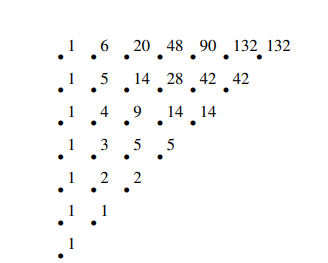
\includegraphics[width=0.5\linewidth]{img/triangulo_catalan.png}
    \caption{Triángulo de Catalán hasta $n = 6$.}
\end{figure}

\subsection{Números de Narayana}

Sean $n, k \in \Z^+$ con $k \leq n$, los números de Narayana se definen como
$$N(n, k) = \frac{1}{n}\binom{n}{k}\binom{n}{k - 1}.$$

Se cumple que
$$N(n, k) = N(n, n - k + 1),$$
$$\sum_{k = 1}^n N(n, k) = C_n,$$

donde $C_n$ es el $n$-ésimo número de Catalán. El número $N(n, k)$ cuenta

\begin{itemize}
    \item La cantidad de secuencias de paréntesis balanceadas con $2n$ paréntesis y $k$ distintos anidamientos, es decir, $k$ ocurrencias de la subcadena $()$.
    \item La cantidad de caminos distintos desde $(0, 0)$ a $(2n, 0)$ dando pasos hacia arriba o abajo y siempre avanzando una unidad en cada paso (diagonales), de manera que haya exactamente $k$ picos. Equivalentemente a la cantidad de maneras de ordenar $n$ $1$'s y $n$ $(-1)$'s en una secuencia $a_i$ tales que si $S_i$ es la suma parcial de $a_i$, entonces $\set{S_i}$ tiene exactamente $k$ máximos locales.
    \begin{figure}[H]
        \centering
        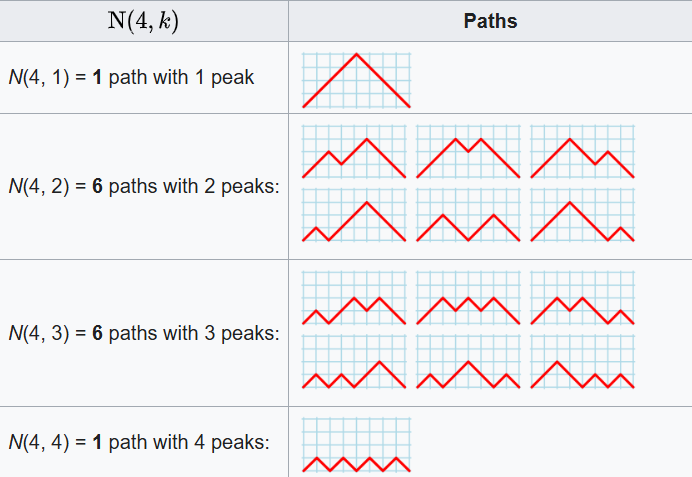
\includegraphics[width=0.5\linewidth]{img/caminos_picos_narayana.png}
        \caption{Caminos de $(0,0)$ a $(8, 0)$ que cuenta $N(4, k)$.}
    \end{figure}
    \item La cantidad de árboles enraizados con $n + 1$ nodos y $k$ hojas.
    \item La cantidad de particiones no cruzadas de un conjunto de tamaño $n$ en exactamente $k$ subconjuntos.
\end{itemize}


\subsection{Particiones Enteras}
Genera todas las particiones de un número \(n\) como suma de enteros positivos en orden no creciente. Complejidad: Tiempo \(O\Pa{ \frac{13^{\sqrt{n}}}{n} }\) – Memoria extra \(O(n)\).

\begin{minted}{cpp}
void generar(int n, int maximo, vi &actual){
    if(n == 0){// Aqui trabajar con actual
        return; }
    for(int i = min(n, maximo); i >= 1; --i){
        actual.pb(i);
        generar(n - i, i, actual);
        actual.pop_back();
    }
}
\end{minted}
La función de partición \( p(n) \), que cuenta el número de formas distintas de escribir \( n \) como suma de enteros positivos sin importar el orden,

% INSERTAR TABLA
\begin{table}[H]
	\centering
	\begin{tabular}{|c|cccccccc|}
		\hline
		$n$ & 1 & 2 & 3 & 4 & 5 & 6 & 7 & 8\\
		\hline
		$p(n)$ & 1 & 2 & 3 & 5 & 7 & 11 & 15 & 22\\
		\hline
		\hline
		$n$ & 9 & 10 & 11 & 12 & 13 & 14 & 15 & 16 \\
		\hline
		 $p(n)$ & 30 & 42 & 56 & 77 & 101 & 135 & 176 & 231\\
		\hline
	\end{tabular}
	\caption{Particiones enteras}
\end{table}

Tiene la siguiente aproximación asintótica para valores grandes de $n$, conocida como la fórmula de Hardy-Ramanujan:

\[
p(n) \sim \frac{1}{4n\sqrt{3}} \exp\left( \pi \sqrt{\frac{2n}{3}} \right)
\]


\hrulefill
\section{Cálculo}
\subsection{Transformada de Fourier}
\textbf{FFT.} Complejidad: Tiempo $O(n\log n)$ - Memoria extra $O(n\log n)$, donde $n$ es el grado del polinomio $P$.
\begin{minted}{cpp}
using comp = complex<double>;
const double PI = acos(-1);
vector<comp> FFT(vector<comp> &P, bool inversa){
    int n = sz(P);
    if(n == 1) return P;
    vector<comp> Pe, Po;
    for(int i = 0; i < n; ++i)
        if(i % 2) Po.pb(P[i]);
        else Pe.pb(P[i]);
    vector<comp> eval_Pe = FFT(Pe, inversa);
    vector<comp> eval_Po = FFT(Po, inversa);
    vector<comp> eval(n);
    double angulo = 2*PI / n * (inversa? -1 : 1);
    comp w(1), w_n(cos(angulo), sin(angulo));
    for(int i = 0; i < n / 2; ++i){
        eval[i] = eval_Pe[i] + w * eval_Po[i];
        eval[i+n/2] = eval_Pe[i] - w*eval_Po[i];
        if(inversa){eval[i]/=2; eval[i+n/2]/=2;}
        w *= w_n;
    } return eval;
}
\end{minted}

\vspace{-1.2\baselineskip}
\hrulefill\\
\textbf{Multiplicar polinomios.} Complejidad: Tiempo $O(n\log n)$ - Memoria extra $O(n\log n)$, donde $n$ es el grado máximo del polinomio $A$ o $B$.
\begin{minted}{cpp}
vi multiplicar(vi A, vi B){
    vector<comp> cA(all(A)), cB(all(B));
    int n = 1;
    while(n < sz(A) + sz(B)) n *= 2;
    cA.resize(n);
    cB.resize(n);
    vector<comp> val_A = FFT(cA, false);
    vector<comp> val_B = FFT(cB, false);
    for(int i=0; i<n; ++i) val_A[i] *= val_B[i];
    val_A = FFT(val_A, true);
    vi res(n);
    for(int i = 0; i < n; ++i)
        res[i] = round(val_A[i].real());
    int carry = 0;
    for(int i = 0; i < n; i++){ res[i] += carry;
        carry = res[i] / 10; res[i] %= 10;
    } return res;
}
\end{minted}


%=%=%=%=%=%=%=%=%=%=%=%=%=%=%=%=%=%=%=%=%=%=%=%=%=%=
%=%=%=%=%=%=%=%=%=%=%=%=%=%=%=%=%=%=%=%=%=%=%=%=%=%=
%=%=%=%=%=%=%=%=%=%=%=%=%=%=%=%=%=%=%=%=%=%=%=%=%=%=
%=%=%=%=%=%=%=%=%=%=%=%=%=%=%=%=%=%=%=%=%=%=%=%=%=%=
\vspace{-1.2\baselineskip}
\hrulefill
\section{Formulazas}

%=%=%=%=%=%=%=%=%=%=%=%=%=%=%=%=%=%=%=%=%=%=%=%=%=%=
%=%=%=%=%=%=%=%=%=%=%=%=%=%=%=%=%=%=%=%=%=%=%=%=%=%=
\subsection{Lógica - Conjuntos - Bitwise}
$\oplus$ es el xor (o diferencia simétrica de conjuntos).
\begin{enumerate}[1.]
    \item $a|b = a\oplus b + a \& b$
    \item $a\oplus (a\&b) = (a|b)\oplus b$
    \item $b\oplus (a\&b) = (a|b)\oplus a$
    \item $(a\&b)\oplus (a|b) = a\oplus b$
    \item $a + b = a|b + a\&b = a\oplus b + 2(a\&b)$
    \item $a - b = (a\oplus (a\&b))-((a|b)\oplus a) = ((a|b)\oplus b)-((a|b)\oplus a)$
    \item $a - b = (a\oplus (a\&b))-(b\oplus (a\&b)) = ((a|b)\oplus b)-(b\oplus (a\&b))$
\end{enumerate}

Si $p, q$ son predicados, entonces:
\begin{enumerate}[1.]
    \item $(p \vee q) \iff -(-p \wedge -q)$.
    \item $(p \implies q) \iff (-p \vee q)$.
    \item $(p \oplus q) \iff -(p \iff q)$.
\end{enumerate}

\subsection{Combinatoria}

\textbf{Inclusión-Exclusión.} Sean $A_1, \dots, A_n$ conjuntos, entonces
$$\abs{\bigcup_{i = 1}^n A_i} = \sum_{\varnothing \neq J \subseteq [n]} (-1)^{|J| - 1}\abs{\bigcap_{j \in J} A_j}$$

\textbf{Cantidad de elementos en exactamente $r$ conjuntos.} Sean $A_1, \dots, A_n$ conjuntos y $0 \leq r \leq n$, la cantidad de elementos en exactamente $r$ conjuntos $A_i$ es
$$\sum_{m = r}^n (-1)^{m - r}\binom{m}{r}\sum_{\substack{J \subseteq [n]\\|J| = m}} \abs{\bigcap_{j \in J} A_j}$$

\textbf{Teorema del binomio generalizado.} Para $x \in \R$ y $a, b \in \mathbb{C}$ se cumple
$$(a + b)^x = \sum_{k = 0}^\infty \binom{x}{k}a^{x}b^{x - k},$$
$$\binom{x}{k} = \frac{1}{k!}\prod_{j = 0}^{k - 1}(x - j) = \frac{x(x - 1)(x - 2)\cdots(x - k + 1)}{k!}.$$

\textbf{ES FIBONACCI} \textit{(En un icpc, el de la Cangurera lo usó)}. En el \textit{Triángulo de Pascal}, los elementos en una ``diagonal'' satisfacen
\[
F_{n+1} = \sum_{k=0}^{\lfloor n/2 \rfloor} \binom{n-k}{k},
\]
donde \( F_{n+1} \) es el \((n+1)\)-ésimo número de Fibonacci.

\begin{figure}[H]
    \centering
	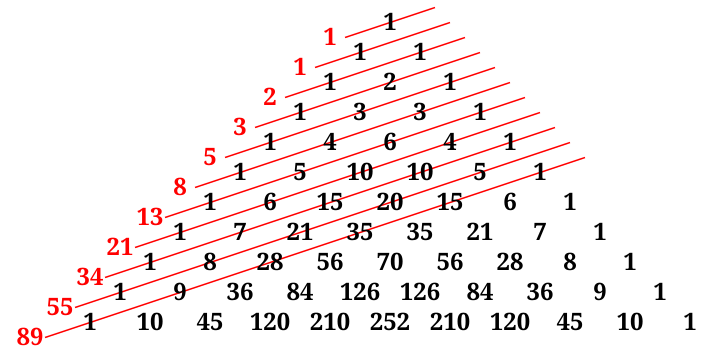
\includegraphics[width=0.5\columnwidth]{img/FiboPascal.png}
\end{figure}

\textbf{Palo de Hockey.}
Para \( n \) y \( r \) \((n \geq r)\), se cumple
\[
\sum_{k=r}^{n} \binom{k}{r} = \binom{n+1}{r+1}.
\]

\textbf{Derangements.} ¿Cuántos trastornos mentales distintos de tamaño $n$ hay? (Según Google Translator). Considera los conjuntos $\set{A_k}_{k = 1}^{k = n}$ donde $A_k$ es la cantidad de permutaciones con el punto fijo $p_k = k$. La cantidad de permutaciones con al menos un punto fijo es
\begin{align*}
	P &:= \abs{\bigcup_{i = 1}^n A_i} = \sum_{\varnothing \neq J \subseteq [n]} (-1)^{|J| - 1}\abs{\bigcap_{j \in J} A_j}\\
	&= \sum_{\varnothing \neq J \subseteq [n]} (-1)^{|J| - 1}(n - |J|)!
	= \sum_{i = 1}^n (-1)^{i - 1}\binom{n}{i}(n - i)!,
\end{align*}

entonces la cantidad de desarreglos es $n! - P$. Si $d_n$ es la cantidad de desarreglos de tamaño $n$ se cumple $d_n = (n - 1)(d_{n  -1} + d_{n - 2})$ con $d_1 = 0$ y $d_0 = d_2 = 1$. También se cumple $d_n = n!d_{n - 1} + (-1)^n$. Sea $0 \leq k \leq n$ y $d_{n, k}$ la cantidad de desarreglos de tamaño $n$ con exactamente $k$ puntos fijos, entonces $d_{n, k} = \binom{n}{k}d_{n - k}$.

%=%=%=%=%=%=%=%=%=%=%=%=%=%=%=%=%=%=%=%=%=%=%=%=%=%=
%=%=%=%=%=%=%=%=%=%=%=%=%=%=%=%=%=%=%=%=%=%=%=%=%=%=
\subsection{Geometría}

\textbf{Teorema de los círculos de Descartes}. Si cuatro círculos son mutuamente tangentes de curvatura $k_i= 1/r_i$ el teorema dice:
\begin{equation*}
    (k_1+k_2+k_3+k_4)^2 = 2\left( k_1^2 +k_2^2 +k_3^2 +k_4^2   \right)
\end{equation*}
\begin{equation*}
    k_4 = k_1+k_2+k_3 \pm 2\sqrt{k_1k_2+k_2k_3+k_3k_1}
\end{equation*}

\textbf{Formula de Heron}. Dado un trinangulo de lados $a, b, c$, escribimos su semiperimetro $s = \frac{a+b+c}{2}$, inradio r, y cuirunradio R.

\begin{equation*}
    Area = \sqrt{s(s-a)(s-b)(s-c)}
\end{equation*}
\begin{equation*}
    2R = \frac{abc}{2  \sqrt{s(s-a)(s-b)(s-c)}}
\end{equation*}
\begin{equation*}
    r =  \sqrt{\frac{(s-a)(s-b)(s-c)}{s} }
\end{equation*}

\textbf{Fórmula de Brahmagupta}. Para el Area se vale algo similar en cuadrilateros ciclicos
\begin{equation*}
    Area = \sqrt{(s-a)(s-b)(s-c)(s-d)}
\end{equation*}

Para no cíclicos, $\theta=$ promedio de dos ángulos opuestos, $p$ y $q$ diagonales
\begin{align*}
    Area &= \sqrt{(s-a)(s-b)(s-c)(s-d)-abcd \cos^2\theta}\\
    &=\sqrt{K},
\end{align*}

donde $K = (s-a)(s-b)(s-c)(s-d) - \frac{1}{4}(ac+bd+pq)(ac+bd-pq)$.

\textbf{Multidimensional} \textit{(Como Chang).} Para más dimensiones, si $A$ es la matriz con filas estos vectores
\begin{equation*}
    Volumen_n = \frac{1}{n!} \sqrt{det\Pa{AA^T}}
\end{equation*}


\hrulefill
\section{Métodos numéricos}
\subsection{Inversa de Matriz con Gauus-Jordan}
Complejidad: Tiempo $O\left(n^3\right)$ - Memoria $O\left(n^2\right)$
\begin{minted}{cpp}
#define eps 0.0001
vector<vector<double>> gauss(vector<vector<double>> m){
    int tam = sz(m);
    vector<vector<double>> id(tam, vector<double>(tam));
    for(int i=0; i<tam; i++) id[i][i] = 1;
    for(int i=0; i<tam; i++){
        // buscar un no 0 para poner en (i,i)
        if(abs(m[i][i]) < eps){
            int j=i+1
            while(abs(m[j][i]) > eps && j<tam){
                swap(m[j], m[i]);
                swap(id[j], id[i]); j++;
            }
            if(j == tam){/*...*/}//no invertible
        }
        /// ponner un uno en (i,i) /// modificar la fila i
        double tmp = m[i][i];
        for(int k=0; k<tam; k++)
            id[i][k] /= tmp, m[i][k] /= tmp;
        /// poner columna i en todo 0, excepto casilla (i,i)
        for(int j=0; j<tam; j++){
            if(j==i) continue;
            //a la fila j le restamos la fila i
            tmp = m[j][i];
            for(int k=0; k<tam; k++){
                m[j][k] = m[j][k]-tmp*m[i][k];
                id[j][k] = id[j][k]-tmp*id[i][k];
            }
        }
    } return id;
}
vector<double> matporvec(vector<vector<double>> &m, vector<double> &b){
    vector<double> ans(sz(b));
    for(int i=0; i<sz(b); i++)
    for(int k=0; k<sz(b); k++)
        ans[i] += m[i][k]*b[k];
    return ans;
}
\end{minted}

\vspace{-1.2\baselineskip}
\hrulefill
\subsection{Sistemas de ecuaciones lineales }
Dado un sistema de $n$ ecuaciones  con $m$ incógnitas. Devuelve el numero de soluciones del sistema $0, \ 1 $ o $\infty$ y si existe al menos una solución la guarda en el vector \mintinline{cpp}{ans}. Complejidad: Tiempo $O(  (n+m)nm ) $ - Memoria $O(nm)$.
\begin{minted}{cpp}
const double EPS = 1e-9;
const int INF = 2; // it doesn't actually have to be infinity or a big number
int gauss(vector<vector<double>> a, vector<double> &ans){
    int n = (int) sz(a);
    int m = (int) sz(a[0]) - 1;
    vi where (m, -1);
    for(int col=0,row=0; col<m && row<n; ++col){
        int sel = row;
        for (int i=row; i<n; ++i)
        if(abs(a[i][col])>abs(a[sel][col]))sel=i;
        if(abs(a[sel][col]) < EPS) continue;
        for(int i=col; i<=m; ++i)
            swap(a[sel][i], a[row][i]);
        where[col] = row;
        for(int i=0; i<n; ++i)
        if(i != row){
            double c = a[i][col] / a[row][col];
            for(int j=col; j<=m; ++j)
                a[i][j] -= a[row][j] * c;
        } ++row;
    } ans.assign (m, 0);
    for(int i=0; i<m; ++i) if(where[i] != -1)
        ans[i] = a[where[i]][m] / a[where[i]][i];
    for(int i=0; i<n; ++i){
        double sum = 0;
        for(int j=0; j<m; ++j)
            sum += ans[j] * a[i][j];
        if(abs(sum - a[i][m]) > EPS) return 0;
    }
    for(int i=0; i<m; ++i) if(where[i] == -1)
        return INF;
    return 1;
}
\end{minted}

\vspace{-1.2\baselineskip}
\hrulefill
\subsection{Sistemas de ecuaciones modulo 2}
Dado un sistema de $n$ ecuaciones  con $m$ incógnitas modulo 2. Devuelve el numero de soluciones del sistema $0, \ 1 $ o $\infty$ y si existe al menos una solución la guarda en el vector \mintinline{cpp}{ans}. Complejidad: Tiempo $O(  (n+m)nm ) $  Memoria $O(nm)$.
\begin{minted}{cpp}
int gauss (vector<bitset<MAXN>> A, int n, int m, bitset<MAXN> &ans){
    // where[i] guarda el indice de la ecaucion donde se puede despejar variable i, -1 si es independiente
    vi where(m, -1);
    //  Matriz "diagonal"
    for(int col=0,row=0; col<m && row<n; ++col){
        // busca pivote
        for(int i = row; i<n; ++i) if(A[i][col]){
            swap (A[i], A[row]);
            break;
        } if(!A[row][col]) continue;
        where[col] = row;
        // poner 0 todos lados
        for(int i=0; i<n; ++i)
        if(i != row && A[i][col]) A[i] ^= A[row];
        ++row;
    }
    // sacar respuesta // variables independientes = 1, t
    for(int i = 0; i < m; ++i)
        ans[i] = where[i] == -1 ? 1 : ((A[where[i]].count() ^ 1) & 1);
    // si hay alguna variable libre
    for(int i = 0; i < m; ++i) if(where[i] == -1)
        return INF;
    return 1;
}
\end{minted}

\vspace{-1.2\baselineskip}
\hrulefill
\section{Sparse table}
Complejidad: Tiempo de precalculo $O(n\log n)$ - Tiempo en responder $O(\log (r - l + 1))$ - Tiempo en responder para operaciones idempotentes $O(1)$ - Memoria extra $O(n\log n)$. \mintinline{cpp}{LOGN} es $\lceil \log_2(\mintinline{cpp}{MAXN}) \rceil$. Indexado en $0$.
\begin{minted}{cpp}
struct sparse_table{
    int n, NEUTRO;
    vvi ST;
    vi lg2;
    int f(int a, int b){return a + b;}
    sparse_table(int _n, int data[]){
        n = _n;
        NEUTRO = 0;
        lg2.resize(n + 1);
        lg2[1] = 0;
        for(int i=2; i<=n; ++i)lg2[i]=lg2[i/2]+1;
        ST.resize(lg2[n] + 1, vi(n + 1, NEUTRO));
        for(int i=0; i<n; ++i)ST[0][i] = data[i];
        for(int k = 1; k <= lg2[n]; ++k){
            int fin = (1 << k) - 1;
            for(int i = 0; i + fin < n; ++i)
            ST[k][i]=f(ST[k-1][i],
                       ST[k-1][i+(1<<(k-1))]);
        }
    }
    int query(int l, int r){
        if(l > r) return NEUTRO;
        int ans = NEUTRO;
        for(int k = lg2[n]; 0 <= k; --k){
            if( r - l + 1 < (1 << k) ) continue;
            ans = f(ans, ST[k][l]);
            l += 1 << k;
        }
        return ans;
    }
    int queryIdem(int l, int r){
        if(l > r) return NEUTRO;
        int lg = lg2[r - l + 1];
        return f(ST[lg][l], ST[lg][r-(1<<lg)+1]);
    }
};
\end{minted}

\vspace{-1.2\baselineskip}
\hrulefill
\section{Fenwick Tree}
Complejidad: Tiempo en responder $O(\log n)$ - Tiempo de actualización $O(\log n)$ - Memoria extra $O(n)$. Indexado en $1$.
\begin{minted}{cpp}
struct fenwick_tree{
    int n;
    vi BIT;
    fenwick_tree(int _n){
        n = _n;
        BIT.resize(n + 1);
    }
    void add(int pos, int x){
        while(pos <= n){
            BIT[pos] += x;
            pos += lsb(pos);
        }
    }
    int sum(int pos){
        int res = 0;
        while(pos){
            res += BIT[pos];
            pos -= lsb(pos);
        } return res;
    }
};
\end{minted}

\vspace{-1.2\baselineskip}
\hrulefill
\section{Segment Tree}
\begin{minted}{cpp}
struct node{
    int val, lazy;
    node():val(0), lazy(0){}
    node(int x, int lz = 0):val(x), lazy(lz){}
    const node operator+(const node &b)const{
        return node(val + b.val);
    }
}
\end{minted}

\vspace{-1.2\baselineskip}
\hrulefill
\subsection{Actualizaciones puntuales}
Complejidad: Tiempo de precalculo $O(n)$ - Tiempo en responder $O(\log n)$ - Tiempo de actualización $O(\log n)$ - Memoria extra $O(n)$. Indexado en $1$.
\begin{minted}{cpp}
struct segment_tree{
    struct node{...};
    vector<node> nodes;
    segment_tree(int n, int data[]){
        nodes.resize(4 * n + 1);
        build(1, n, data);
    }
    void build(int left, int right, int data[], int pos = 1){
        if(left == right){
            nodes[pos] = node(data[left]);
            return;
        }
        int mid = (left + right) / 2;
        build(left, mid, data, pos * 2);
        build(mid + 1, right, data, pos * 2 + 1);
        nodes[pos] = nodes[pos*2]+nodes[pos*2+1];
    }
    void update(int x, int idx, int left, int right, int pos = 1){
        if(idx < left || right < idx) return;
        if(left == right){
            nodes[pos].val += x;
            return;
        }
        int mid = (left + right) / 2;
        update(x, idx, left, mid, pos * 2);
        update(x, idx, mid+1, right, pos*2+1);
        nodes[pos] = nodes[pos*2]+nodes[pos*2+1];
    }
    node query(int l, int r, int left, int right, int pos = 1){
        if(r < left || right < l) return node();
        if(l <= left && right <= r)
            return nodes[pos];
        int mid = (left + right) / 2;
        return query(l, r, left, mid, pos*2) + query(l, r, mid+1, right, pos*2+1);
    }
};
\end{minted}

\vspace{-1.2\baselineskip}
\hrulefill
\subsection{Actualizaciones sobre rangos}
Complejidad: Tiempo de precalculo $O(n)$ - Tiempo en responder $O(\log n)$ - Tiempo de actualización $O(\log n)$ - Memoria extra $O(n)$.
\begin{minted}{cpp}
struct segment_tree{
    struct node{...};
    vector<node> nodes;
    segment_tree(int n, int data[]){...}
    void build(...){...}
    void combine_lz(int lz, int pos){nodes[pos].lazy += lz;}
    void apply_lz(int pos, int tam){
        nodes[pos].val += nodes[pos].lazy * tam;
        nodes[pos].lazy = 0;
    }
    void push_lz(int pos, int left, int right){
        int len = abs(right - left + 1);
        if(1 < len){
            combine_lz(nodes[pos].lazy, pos*2);
            combine_lz(nodes[pos].lazy, pos*2+1);
        } apply_lz(pos, len);
    }
    void update(int x, int l, int r, int left, int right, int pos = 1){
        push_lz(pos, left, right);
        if(r < left || right < l) return;
        if(l <= left && right <= r){
            combine_lazy(x, pos);
            push_lazy(pos, left, right);
            return;
        }
        int mid = (left + right) / 2;
        update(x, l, r, left, mid, pos * 2);
        update(x, l, r, mid+1, right, pos*2+1);
        nodes[pos] = nodes[pos*2]+nodes[pos*2+1];
    }
    node query(int l, int r, int left, int right, int pos = 1){
        push_lz(pos, left, right);
        ...
    }
};
\end{minted}

\vspace{-1.2\baselineskip}
\hrulefill
\subsection{Sparse segment tree}
\begin{minted}{cpp}
struct node{
    ll lazy, maxi, sum;
    node *left = nullptr, *right = nullptr;
    node(): lazy(0), maxi(0), sum(0){}
    void extend(){
        if(left) return;
        left = new node;
        right = new node;
    }
    void combine_lz(ll lz){
        lazy += lz;
    }
    void apply_lz(ll len){
        sum += len * lazy; lazy = 0;}
    void push_lz(ll L, ll R){
        int len = R - L + 1;
        ll mid = L + (R - L) / 2;
        if(len){
            extend();
            left->combine_lz(lazy);
            right->combine_lz(lazy);
        }
        apply_lz(len);
    }
    void update(ll x, ll l, ll r, ll L, ll R){
        push_lz(L, R);
        if(r < L || R < l) return;
        if(l <= L && R <= r){
            combine_lz(x);
            push_lz(L, R);
            return;
        }
        ll mid = L + (R - L) / 2;
        extend();
        left->update(x, l, r, L, mid);
        right->update(x, l, r, mid + 1, R);
        sum = left->sum + right->sum;
    }
    ll query(ll l, ll r, ll L, ll R){
        push_lz(L, R);
        if(r < L || R < l) return 0;
        if(l <= L && R <= r) return sum;
        extend();
        ll mid = L + (R - L) / 2;
        return left->query(l, r, L, mid) + right->query(l, r, mid + 1, R);
    }
};
\end{minted}

\vspace{-1.2\baselineskip}
\hrulefill
\section{Sqrt decomposition}
\subsection{Algoritmo de MO}
Complejidad: Tiempo en responder $O((n + q)\sqrt{n}F + q\log q)$, donde $O(F)$ es la complejidad de \mintinline{cpp}{add()} y \mintinline{cpp}{remove()}.
\begin{minted}{cpp}
const int block_size = 300;
struct query {
    int l, r;
    int block, i;
    bool operator<(const query &b) const {
        if(block == b.block) return r < b.r;
        return block < b.block;
    }
};
void add(int idx){/// TO-DO}
void remove(int idx){/// TO-DO}
int get_answer(){return 0; /// TO-DO}
vi solve(vector<query> &queries) {
    vi answers(sz(queries));
    sort(queries.begin(), queries.end());
    int cur_l = 0, cur_r = -1;
    for(query q : queries){
        while(cur_l > q.l) add(--cur_l);
        while(cur_r < q.r) add(++cur_r);
        while(cur_l < q.l) remove(cur_l++);
        while(cur_r > q.r) remove(cur_r--);
        answers[q.i] = get_answer();
    } return answers;
}
\end{minted}

%\bigskip
% \section{DSU}
% Complejidad: Tiempo $O(\log(n))$ - Memoria $O(n)$, donde $n$ es la cantidad total de elementos. La complejidad temporal es por cada función.
% \par \mintinline{cpp}{P[MAXN]}: guarda el representante para cada nodo.
% \par \mintinline{cpp}{RA[MAXN]}: guarda el rango (peso) del conjunto de cada representante para el \textit{small to large}.
% \begin{minted}{cpp}
% struct dsu{
%     struct action{
%         int x_p, y_p, rank_y;
%     };
%     vi RA, P;
%     vector<action> actions;
%     dsu(int n){
%         RA.resize(n, 1);
%         P.resize(n);
%         iota(P.begin(), P.end(), 0);
%     }
%     int root(int x){
%         return x == P[x] ? x : P[x] = root(P[x]);
%     }
%     bool join(int x, int y, bool recording){
%         x = root(x);
%         y = root(y);
%         if(x == y) return false;
%         if(RA[x] >= RA[y]) swap(x, y);
%         if(recording) actions.pb({x, y, RA[y]});
%         RA[y] += RA[x];
%         P[x] = y;
%         return true;
%     }
%     void rollback(int cnt){
%         while(cnt-- > 0 && actions.size()){
%             action act = actions.back();
%             actions.pop_back();
%             RA[act.y_p] = act.rank_y;
%             P[act.x_p] = act.x_p;
%         }
%     }
% };
% \end{minted}

%\bigskip
%\newpage
\vspace{-1.2\baselineskip}
\hrulefill
\section{Grafos}
\begin{minted}{cpp}
struct edge{
    int from, to;
    ll w;
    const bool operator<(const edge &b)const{
        return w > b.w;
    }
};
struct pos{
    int from;
    ll c;
    const bool operator<(const pos &b)const{
        return c > b.c;
    }
};
\end{minted}

\vspace{-\baselineskip}
\hrulefill
\subsection{Caminos mínimos}
\textbf{Dijkstra.} Complejidad: Tiempo $O(|E| \log |V|)$ - Memoria extra $O(|E|)$.
\begin{minted}{cpp}
ll dijkstra(int a, int b, vector<edge> graph[]){
    ll dist[MAXN];
    bool vis[MAXN] = {};
    fill(dist, dist + MAXN, LLONG_MAX);
    priority_queue<pos> q;
    q.push(pos{a, 0});
    dist[a] = 0;
    while(!q.empty()){
        pos act = q.top();
        q.pop();
        if(vis[act.from]) continue;
        vis[act.from] = true;
        for(edge &e : graph[act.from]){
            if(dist[e.to] <= dist[e.from] + e.w) continue;
            dist[e.to] = dist[e.from] + e.w;
            q.push(pos{e.to, dist[e.to]});
        }
    } return dist[b];
}
\end{minted}

\vspace{-1.2\baselineskip}
\hrulefill\\
\textbf{Bellman-Ford.} Complejidad: $O(\abs{V}\abs{E})$.
\begin{minted}{cpp}
vi bellman_ford(int s, int n, vector<edge> &edges, bool cycles = false){
    vi d(n, (cycles ? 0 : INT_MAX));
    d[s] = 0;
    vi P(n, -1); /// Predecesor
    for(int i = 0; i < n - 1; ++i)
    for(edge &e : edges){
        if(d[e.from] == INT_MAX) continue;
        if(d[e.to] > d[e.from] + e.w){
            d[e.to] = d[e.from] + e.w;
            P[e.to] = e.from;
        }
    }
    int last_relax = -1;
    for(edge &e : edges){
        if(d[e.from] == INT_MAX) continue;
        if(d[e.to] > d[e.from] + e.w){
            d[e.to] = d[e.from] + e.w;
            P[e.to] = e.from;
            last_relax = e.to;
        }
    }
    if(last_relax == -1) return d;
    return {}; /// VACIO
}
\end{minted}

\vspace{-1.2\baselineskip}
\hrulefill \\
\textbf{Floyd-Warshall.} Complejidad: $O\pa{\abs{V}^3}$.
\begin{minted}{cpp}
vvi floyd_warshall(int n){
    const int INF = INT_MAX; // para evitar overflow después
    vvi d(n, vi(n, INF));
    /// aqui inicializa con la lista/matriz de adyacencia
    /// luego calcula la dp
    for(int k = 0; k < n; ++k){
        for(int i = 0; i < n; ++i){
            for(int j = 0; j < n; ++j){
                if(d[i][k]==INF || d[k][j]==INF)
                    continue;
                if(d[i][j] > d[i][k] + d[k][j]) d[i][j] = d[i][k] + d[k][j];
            }
        }
    } return d;
}
\end{minted}

\vspace{-1.2\baselineskip}
\hrulefill\\
\textbf{Johnson's algorithm.} Complejidad: $O(\abs{V}\abs{E}\log\abs{V})$. Sea $p: V \to \R$ una función potencial del grafo. El algoritmo es como sigue:
\begin{enumerate}[1.]
    \item Hacemos una transformación en el grafo cambiando los pesos $w$ a $w'(u, v) = w(u, v) + p(u) - p(v)$.
    \item Calculamos la distancia mínima $d': V \times V \to \R$ desde cada nodo a todos los demás con Dijkstra.
    \item Finalmente, la distancia mínima de $u$ a $v$ en el grafo original es $d(u, v) = d'(u, v) - p(u) + p(v)$.
\end{enumerate}
La función potencial $p$ puede ser cualquiera. Usando Bellman-Ford se puede calcular el potencial $p(u)$ como el camino más corto que termina (o empieza) en $u$.

\hrulefill
\subsection{Árboles}
\textbf{Prim.} Complejidad: Tiempo $O(|E| \log |V|)$. \mintinline{cpp}{eCost[MAXN]} es el arreglo de costos mínimos de cada nodo para incluirlo en el MST.
\begin{minted}{cpp}
ll prim(vector<edge> graph[]){
    ll e_cost[MAXN], ans = 0;
    bool vis[MAXN] = {};
    fill(e_cost, e_cost + MAXN, LLONG_MAX);
    priority_queue<edge> q;
    q.push(edge{1, 1, 0});
    while(sz(q)){
        int node = q.top().to;
        ll w = q.top().w; q.pop();
        if(vis[node]) continue; vis[node] = true;
        for(edge &e : graph[node]){
            if(vis[e.to] || e_cost[e.to] <= e.w) continue;
            e_cost[e.to] = e.w;
            q.push(e);
        } ans += w;
    } return ans;
}
\end{minted}

\vspace{-1.2\baselineskip}
\hrulefill\\
\textbf{Kruskal.} Complejidad: Tiempo $O\pa{|E|\log |E|}$.
\begin{minted}{cpp}
ll kruskal(vector<edge> &edges, int n){
    sort(all(edges));
    dsu mset(n);
    ll res = 0;
    for(edge &e : edges){
        if(mset.root(e.from) == mset.root(e.to)) continue;
        mset.join(e.from, e.to);
        res += e.w;
    }
    return res;
}
\end{minted}

\vspace{-1.2\baselineskip}
\hrulefill\\
\textbf{Boruvka.} Complejidad: Tiempo $O\pa{|E|\log |V|}$. $|V| = n$. \mintinline{cpp}{dsu.join()} devuelve \mintinline{cpp}{true} si la unión se llevó a cabo o \mintinline{cpp}{false} en otro caso.
\begin{minted}{cpp}
ll boruvka(vector<edge> &edges, int n){
    dsu mset(n);
    int min_edge[n];
    ll res = 0;
    while(mset.cnt_comp > 1){
        fill(min_edge, min_edge + n, -1);
        for(int i = 0; i < sz(edges); ++i){
            int u = mset.root(edges[i].from);
            int v = mset.root(edges[i].to);
            if(u == v) continue;
            if(min_edge[u] == -1 || edges[i].w < edges[min_edge[u]].w) min_edge[u] = i;
            if(min_edge[v] == -1 || edges[i].w < edges[min_edge[v]].w) min_edge[v] = i;
        }
        for(int i = 0; i < n; ++i){
            int idx_e = min_edge[i];
            if(idx_e == -1) continue;
            res += mset.join(edges[idx_e].from, edges[idx_e].to) * edges[idx_e].w;
        }
    } return res;
}
\end{minted}

\vspace{-1.2\baselineskip}
\hrulefill\\
\textbf{MST dirigido.} Complejidad: $O(|E|\log|V|)$. AGREGAR PEQUEÑA DESCRIPCIÓN.
\begin{minted}{cpp}
/// MEJORAR ESTA COSA, SOLO LO COPIE Y PEGUÉ porcuestionesdetiempo
const int N = 3e5 + 9;
const ll inf = 1e18;
template<typename T> struct PQ {
    ll sum = 0;
    priority_queue<T, vector<T>, greater<T>> Q;
    void push(T x) { x.w -= sum; Q.push(x); }
    T pop() { auto ans = Q.top(); Q.pop(); ans.w += sum; return ans; }
    int size() { return sz(Q); }
    void add(ll x) { sum += x; }
    void merge(PQ &x){
        if (size() < sz(x)){
            swap(sum, x.sum);
            Q.swap(x.Q);
        }
        while(sz(x)){
            auto tmp = x.pop();
            tmp.w -= sum;
            Q.push(tmp);
        }
    }
};
struct edge {
    int u, v; ll w;
    bool operator > (const edge &rhs) const { return w > rhs.w; }
};
struct DSU {
    vi par;
    DSU (int n) : par(n, -1) {}
    int root(int i) { return par[i] < 0 ? i : par[i] = root(par[i]); }
    void set_par(int c, int p) { par[c] = p; }
};
// returns parents of each vertex
// each edge should be distinct
// it assumes that a solution exists (all vertices are reachable from root)
// 0 indexed
// Takes ~300ms for n = 2e5
vi DMST(int n, int root, const vector<edge> &edges) {
    vi u(2 * n - 1, -1), par(2 * n - 1, -1);
    edge par_edge[2 * n - 1];
    vi child[2 * n - 1];
    PQ<edge> Q[2 * n - 1];
    for(auto e : edges) Q[e.v].push(e);
    for(int i = 0; i < n; i++)
        Q[(i+1) % n].push({i, (i+1) % n, inf});
    int super = n;
    DSU dsu(2 * n - 1);
    int head = 0;
    while(sz(Q[head])) {
        auto x = Q[head].pop();
        int nxt_root = dsu.root(x.u);
        if (nxt_root == head) continue;
        u[head] = nxt_root;
        par_edge[head] = x;
        if (u[nxt_root] == -1) head = nxt_root;
        else {
            int j = nxt_root;
            do {
                Q[j].add(-par_edge[j].w);
                //Q[super].merge(move(Q[j]));
                Q[super].merge(Q[j]);
                assert(u[j] != -1);
                child[super].pb(j);
                j = dsu.root(u[j]);
            } while (j != nxt_root);
            for(auto u : child[super]) par[u] = super, dsu.set_par(u, super);
            head = super++;
        }
    }
    vi res(2 * n - 1, -1);
    queue<int> q; q.push(root);
    while (sz(q)) {
        int u = q.front();
        q.pop();
        while (par[u] != -1) {
            for (auto v : child[par[u]]) {
                if (v != u) {
                    res[par_edge[v].v] = par_edge[v].u;
                    q.push(par_edge[v].v);
                    par[v] = -1;
                }
            }
            u = par[u];
        }
    }
    res[root] = root; res.resize(n);
    return res;
}
int main() {
    ios_base::sync_with_stdio(0); cin.tie(0);
    int n, m, root; cin >> n >> m >> root;
    vector<edge> edges(m);
    for(auto &e : edges) cin >> e.u >> e.v >> e.w;
    auto res = DMST(n, root, edges);
    unordered_map<int, int> W[n];
    for (auto u : edges) W[u.v][u.u] = u.w;
    ll ans = 0;
    for(int i = 0; i < n; i++) if(i != root)
        ans += W[i][res[i]];
    cout << ans << '\n';
    for(auto x : res) cout << x << ' ';
    cout << '\n';
}
\end{minted}

\vspace{-1.2\baselineskip}
\hrulefill\\
\textbf{Block-Cut Tree} Complejidad: $O(n)$?
\begin{minted}{cpp}
/// MEJORAR ESTA COSA, SOLO LO COPIE Y PEGUÉ porcuestionesdetiempo
vvi comps;//nodes in each component
vvi bcc;//nodes to components that it belong
vi st;//internal stack
vi low, num;
int id;
int sz;
void dfs_biconnected(vvi &g, int u, int pre){
  low[u] = num[u] = ++id;
  st.pb(u);
  for(auto v: g[u]) {
    if(!num[v]) {
      dfs_biconnected(g, v, u);
      low[u] = min(low[u], low[v]);
      if(low[v] >= num[u]) {
        int x;
        comps.pb(vi());
        do {
          x = st.back();
          st.pop_back();
          bcc[x].pb(sz);
          comps.back().pb(x);
        } while(x ^ v);
        bcc[u].pb(sz);
        comps.back().pb(u);
        sz++;
      }
    } else if(v != pre) low[u] = min(low[u], num[v]);
  }
}
vi utoubt;//its component or its AP index
vb uisart;//u is AP?
vvi bt;//block cut tree
void generateBlockCutTree(vvi &g){
    int n = sz(g);
    sz = id = 0;
    bcc.resize(0); low.resize(0); num.resize(0);
    bcc.resize(n); low.resize(n); num.resize(n);
    dfs_biconnected(g, 0, 0);
    bt.resize(sz);
    utoubt.resize(0); utoubt.resize(n);
    uisart.resize(0); uisart.resize(n);
    for(int u = 0; u < n; u++){
        if(sz(bcc[u]) > 1) { //Articulation
            utoubt[u] = sz++;
            uisart[u] = true;
            bt.pb(vi());
            for(auto v: bcc[u]){
                bt[utoubt[u]].pb(v);
                bt[v].pb(utoubt[u]);
            }
        } else //Not articulation point
            utoubt[u] = bcc[u][0];
    }
}
\end{minted}

\vspace{-1.2\baselineskip}
\hrulefill\\
\textbf{LCA.} Complejidad: Tiempo de preproceso $O(|V|\log |V|)$. Tiempo de LCA y $n$-ésimo ancestro $O(\log |V|)$. $1$-index.
\begin{minted}{cpp}
void precalc(int node, int p = 0, int d = 1){
    depth[node] = d;
    P[0][node] = p;
    for(int k = 1; k <= LOGN; ++k)
        P[k][node] = P[k - 1][P[k - 1][node]];
    for(int child : tree[node]) if(p != child)
        precalc(child, node, d + 1);
}
int LCA(int a, int b){
    if(depth[b] < depth[a]) swap(a, b);
    int dif = depth[b] - depth[a];
    for(int k = LOGN; 0 <= k; --k)
        if(is_on(dif, k)) b = P[k][b];
    if(a == b) return a;
    for(int k = LOGN; 0 <= k; --k){
        if(P[k][a] != P[k][b]){
            a = P[k][a];
            b = P[k][b];
        }
    }
    return P[0][a];
}
int nth_ancestor(int u, int n){
    for(int k = LOGN; 0 <= k; --k)
        if(is_on(n, k)) u = P[k][u];
    return u;
}
\end{minted}

\vspace{-1.2\baselineskip}
\hrulefill\\
\textbf{Sack.} Complejidad: Tiempo $O(\abs{V}\log \abs{V})$. $1$-index.
\begin{minted}{cpp}
void precalc(int node, int p = 0){
    subtree_size[node] = 1;
    depth[node] = depth[p] + 1;
    for(int v : tree[node]){
        if(v == p) continue;
        precalc(v, node);
        subtree_size[node] += subtree_size[v];
    }
}
void add(int node, int x, int p = 0){
    /// add node here
    /// add subtree
    for(int v: tree[node])
        if(v != p && !big[v])
            add(v, x, node);
}
void dfs(int node, bool keep, int p = 0){
    int maxi = -1, big_child = -1;
    for(int v : tree[node])///Searchfor big_child
       if(v != p && subtree_size[v] > maxi)
          maxi = subtree_size[v], big_child = v;
    for(int v : tree[node])
        if(v != p && v != big_child)
            dfs(v, false, node);  /// run a dfs on small childs and clear them
    if(big_child != -1)
        dfs(big_child, true, node), big[big_child] = 1;  /// big_child marked as big and not cleared
    add(node, 1, p);
    /// answer queries here
    if(big_child != -1) big[big_child] = 0;
    if(!keep) add(node, -1, p);
}
\end{minted}

\vspace{-1.2\baselineskip}
\hrulefill
\subsection{Máximo flujo}

\textbf{Algunos problemas de flujos}
\begin{itemize}
    \item \textit{Maximum Weight Closure}. Sea $N_1$ una clausura de $G$ y $N_2 = V \setminus N_1$, tenemos que $w\pa{N_1} = \sum_{i \in N_1^+} w_i - \sum_{i \in N_1^-} |w_i|$ y $Cap.Corte = \sum_{i \in N_2^+} w_i + \sum_{i \in N_1^-} |w_i|$. Entonces
    $$Cap.Corte + w(N_1) = \sum_{i \in N_1^+} w_i + \sum_{i \in N_2^+} w_i.$$
    \item \textit{Mínima cobertura de vértices}. En grafos generales es NP-Completo. En grafos bipartitos el máximo emparejamiento es igual al numero de vertices en la mínima cobertura. Para el problema con pesos en los nodos, unimos $s$ a todos los nodos en $L$ con capacidad igual al peso de cada nodo, unimos los nodos de $R$ a $t$ de la misma manera y unimos los nodos de $L$ a $R$ con capacidad infinita. El máximo flujo es el peso mínimo de la mínima cobertura.
    \item \textit{Máximo conjunto independiente}. Cualquier conjunto independiente es el complemento de alguna cobertura de vértices.
    \item \textit{Mínimo cubrimiento de caminos independientes}. En grafos generales es NP-hard. En DAG's duplicamos los nodos en un lado IN y un lado OUT. Conectamos $s$ al lado OUT y el lado IN a $t$. Las aristas del DAG las agregamos del lado OUT al lado IN. Sea $M$ el máximo emparejamiento de la red anterior, entonces el mínimo cubrimiento es $\abs{V} - M$.
    \item \textit{Mínimo cubrimiento de caminos NO necesariamente independientes}. En grafos generales es NP-hard. En DAG's transformamos el DAG a su clausura transitiva y aplicamos el problema anterior.
    \item \textit{Teorema de Mirsky}. En todo POSET, el tamaño de la cadena de mayor tamaño es igual al número de anticadenas necesarias para cubrir todos los elementos del conjunto.
    \item \textit{Teorema de Dilworth}. En todo POSET, el tamaño de la anticadena de mayor tamaño es igual al número de cadenas necesarias para cubrir todos los elementos del conjunto.
    \item \textit{Teorema de Hall}. Un grafo bipartito con subconjuntos $L$ y $R$ tiene un emparejamiento de tamaño $|L|$ si y sólo si para todo subconjunto $W$ de $L$, se cumple que $|W| \leq |N_G(W)|$, donde $N_G(W)$ es el conjunto de vértices vecinos de alguno de los vértices en $W$.
\end{itemize}

\hrulefill\\
\textbf{Edmonds-Karp}
Complejidad: Ford-Fulkerson $O(|E| \cdot F)$, Edmonds-Karp $O(\abs{V}\abs{E}^2)$.
\begin{minted}{cpp}
struct edge {
    int from, to;
    ll w, c, f;
    // weight, capacity, flow
};
class ford_fulkerson {
public:
    ford_fulkerson (vector<vector<edge>> &graph) : graph(graph){}
    ll get_max_flow(int s, int t){
        init();
        ll f = 0;
        while(find_and_update(s, t, f)){}
        return f;
    }
    vi get_st_cut(const int &s){
        bool vis[sz(graph)] = {};
        vi S;
        queue<int> q;
        q.push(s);
        S.pb(s);
        vis[s] = true;
        while(sz(q)){
            int u = q.front(); q.pop();
            for(int eI : edge_indexes[u]){
                if(edges[eI].c > edges[eI].f && !vis[edges[eI].to]){
                    q.push(edges[eI].to);
                    vis[edges[eI].to] = true;
                    S.pb(edges[eI].to);
                }
            }
        }
        return S;
    }
    vector<vector<edge>> get_residual_graph(){
        vector<vector<edge>> residual(sz(graph));
        for(int i=0; i<sz(edges); i+=2){
            const edge& e = edges[i];
            if(e.c > 0){
                residual[e.from].pb({e.from, e.to, e.w, e.c - e.f, e.f});
                residual[e.to].pb({e.to, e.from, -e.w, e.f, -e.f});
            }
        } return residual;
    }
private:
    vector<vector<edge>> graph;
    vector<edge> edges;
    vvi edge_indexes;
    void init(){
      edges.clear();
      edge_indexes.clear();
      edge_indexes.resize(sz(graph));
      for(int u = 0; u < sz(graph); u++){
         for(edge &e : graph[u]){
           edges.pb({u, e.to, e.w, e.c, 0});
           edges.pb({e.to, u, -e.w, 0, 0});
           edge_indexes[u].pb(sz(edges)-2);
           edge_indexes[e.to].pb(sz(edges)-1);
         }
      }
    }
    bool find_and_update(int s, int t, ll &flow){
        queue<int> q;
        // Desde donde llego y con que arista
        vpii from(sz(graph), {-1, -1});
        q.push(s);
        from[s] = {s, -1};
        bool found = 0;
        while(sz(q) && !found){
            int u = q.front(); q.pop();
            for(int eI : edge_indexes[u]){
                if(edges[eI].c > edges[eI].f &&
                  from[edges[eI].to].first== -1){
                    from[edges[eI].to] = {u, eI};
                    q.push(edges[eI].to);
                    if(edges[eI].to == t)found=1;
                }
            }
        }
        if(!found) return false;
        ll u_flow = LLONG_MAX;
        int cur = t;
        while(cur != s) {
            u_flow = min(u_flow, edges[from[cur].se].c - edges[from[cur].se].f);
            cur = from[cur].fi;
        }
        cur = t;
        while(cur != s){
            edges[from[cur].se].f += u_flow;
            edges[from[cur].se^1].f -= u_flow;
            cur = from[cur].fi;
        }
        flow += u_flow;
        return 1;
    }
};
\end{minted}

\vspace{-1.2\baselineskip}
\hrulefill\\
\textbf{Dinic.} Complejidad: $O(\abs{V}^2\abs{E})$.
\begin{minted}{cpp}
const int MAXV = 32767; /// 2^15 - 1
template<class T = ll> struct dinic{
    dinic(short V){this->V = V;}
    const static bool SCALING = 1;
    bool sorted = 0;
    short s, t, V;
    int lim = 1; /// Para escalado
    const T INF = numeric_limits<T>::max();
    short level[MAXV]; /// distancia desde s
    short ptr[MAXV]; /// arista que va explorando
    struct edge{
        short to, rev;
        T cap, flow, mcap;
        bool operator<(const edge &b)const{return mcap > b.mcap;}
    };
    vector<edge> adj[MAXV];
    vi adj_cur[MAXV]; /// aristas del grafo de nivel
    void add_edge(short u, short v, T cap, bool is_directed = 1){
        if(u == v) return;
        T add = (is_directed ? 0 : cap);
        adj[u].pb({v, sz(adj[v]), cap, 0 ,cap+add});
        adj[v].pb({u, sz(adj[u])-1, add, 0, cap+add});
    }
    void mysort(){
        if(sorted) return;
        sorted = 1;
        for(int i = 0; i < V; ++i){
            sort(all(adj[i]));
            for(int j=0; j<sz(adj[i]); ++j)
            adj[adj[i][j].to][adj[i][j].rev].rev = j;
        }
    }
    bool bfs(){
        for(int i = 0; i < V; ++i){
            adj_cur[i].clear();
            adj_cur[i].reserve(sz(adj[i]));
        }
        queue<short> q;
        q.push(s);
        fill(level, level + V, -1);
        level[s] = 0;
        while(sz(q)){
            short u = q.front(); q.pop();
            if(u == t) return 1;
            for(int i=0; i < sz(adj[u]); ++i){
                edge &e = adj[u][i];
                if(e.mcap < lim) break;
                if(level[e.to] == -1 && e.cap - e.flow >= lim){
                    level[e.to] = level[u] + 1;
                    adj_cur[u].pb(i);
                    q.push(e.to);
                } else if(level[e.to]==level[u]+1 && e.cap - e.flow >= lim){
                    adj_cur[u].pb(i);
                }
            }
        } return 0;
    }
    T dfs(short u, T flow, vector<short> &S, bool save = 0){
        if(save) S.pb(u);
        if(u == t) return flow;
        for(; ptr[u] < sz(adj_cur[u]); ++ptr[u]){
            edge &e = adj[u][adj_cur[u][ptr[u]]];
            if(T pushed = dfs(e.to, min(flow, e.cap - e.flow), S, save)){
                e.flow += pushed;
                adj[e.to][e.rev].flow -= pushed;
                if(e.cap-e.flow < lim) ptr[u]++;
                return pushed;
            }
        } return 0;
    }
    ll get_max_flow(short source, short sink){
        s = source; t = sink;
        mysort();
        vector<short> S;
        ll flow = 0;
        lim = SCALING ? (1<<30) : 1;
        for(; 0 < lim; lim >>= 1){
            while(bfs()){
                memset(ptr, 0, sizeof(ptr));
                while(T pushed = dfs(s, INF, S))
                    flow += pushed;
            }
        } return flow;
    }
    vector<short> get_st_cut(){
        vector<short> S;
        memset(ptr, 0, sizeof(ptr));
        dfs(s, INF, S, true);
        return S;
    }
};
\end{minted}

\vspace{-1.2\baselineskip}
\hrulefill\\
\textbf{MCMF.} Complejidad: $O(\min\{|E|^2|V|\log |V|, \; F|E|\log |V|\}).$
\begin{minted}{cpp}
const int MAXV = (1 << 15) - 1;
template<class T = ll> struct mcmf{
    mcmf(short V){this->V = V;}
    short s, t, V;
    const T INF = numeric_limits<T>::max();
    vector<T> p;
    struct edge{
        short to, rev;
        T cap, flow, mcap, w;
        bool operator<(const edge &b)const{return mcap > b.mcap;}
    };
    vector<edge> adj[MAXV];
    void add_edge(short u, short v, T cap, T w, bool is_directed = 1){
        if(u == v) return;
        T add = (is_directed ? 0 : cap);
        adj[u].pb({v, sz(adj[v]), cap, 0, cap + add, w});
        adj[v].pb({u, sz(adj[u]) - 1, add, 0, cap + add, -w});
    }
    struct pos{
        short from;
        T c;
        const bool operator<(const pos &b)const{return c > b.c;}
    };
    vector<T> bellman_ford(){
        vector<T> d(V);
        for(int i = 0; i < V - 1; ++i){
            for(int u = 0; u < V; ++u){
                for(edge &e : adj[u]){
                    if(d[e.to] > d[u] + e.w && e.cap > 0){
                        d[e.to] = d[u] + e.w;
                    }
                }
            }
        } return d;
    }
    pair<T, T> dijkstra(const T MAX_FLOW){
        vector<T> d(V, INF);
        vi P(V, -1), P_e(V, -1);
        priority_queue<pos> q;
        q.push({s, 0});
        d[s] = 0;
        while(sz(q)){
            pos act = q.top(); q.pop();
            if(act.c != d[act.from]) continue;
            for(int j=0; j<sz(adj[act.from]); ++j){
                edge &e = adj[act.from][j];
                if(e.cap - e.flow <= 0) continue;
                T _w = e.w+p[act.from] - p[e.to];
                if(d[e.to] <= d[act.from] + _w)
                    continue;
                d[e.to] = d[act.from] + _w;
                q.push(pos{e.to, d[e.to]});
                P[e.to] = act.from;
                P_e[e.to] = j;
            }
        }
        for(int i = 0; i < V; ++i) if(d[i] < INF)
            d[i] += -p[s] + p[i];
        for(int i = 0; i < V; ++i) if(d[i] < INF)
            p[i] = d[i];
        if(P[t] == -1) return {0, 0};
        T flow = MAX_FLOW;
        int cur_node = t;
        while(cur_node != s){
            flow = min(flow, adj[ P[cur_node] ][ P_e[cur_node] ].cap - adj[ P[cur_node] ][ P_e[cur_node] ].flow);
            cur_node = P[cur_node];
        }
        T new_cost = 0;
        cur_node = t;
        while(cur_node != s){
            adj[ P[cur_node] ][ P_e[cur_node] ].flow += flow;
            new_cost += adj[ P[cur_node] ][ P_e[cur_node] ].w * flow;
            adj[cur_node][adj[ P[cur_node] ][ P_e[cur_node] ].rev ].flow -= flow;
            cur_node = P[cur_node];
        }
        return {flow, new_cost};
    }
    pair<T, T> get_max_flow(short source, short sink, const T MAX_FLOW = 1e8){
        s = source;
        t = sink;
        p = bellman_ford();
        T flow = 0, cost = 0;
        while(flow < MAX_FLOW){
            pair<T, T> pushed = dijkstra(MAX_FLOW - flow);
            if(!pushed.first) break;
            flow += pushed.first;
            cost += pushed.second;
        }
        return {flow, cost};
    }
};
\end{minted}

\vspace{-1.2\baselineskip}
\hrulefill
\subsection{SCC}
\textbf{Kosajaru}
Complejidad: Tiempo $O(n)$.
\begin{minted}{cpp}
void dfs(int node, vi graph[], bool vis[], vi &topo_ord){
    if(vis[node]) return;
    vis[node] = true;
    for(int v : graph[node])
        dfs(v, graph, vis, topo_ord);
    topo_ord.pb(node);
}
void assign_scc(int node, vi inv_graph[], bool vis[], vi &scc, const int id){
    if(vis[node]) return;
    vis[node] = true;
    scc[node] = id;
    for(int v : inv_graph[node])
        assign_scc(v, inv_graph, vis, scc, id);
}
pair<int, vi> kosajaru(int n, vi graph[], vi inv_graph[]){
    bool vis[n] = {};
    vi topo_ord;
    for(int i = 0; i < n; ++i)
        dfs(i, graph, vis, topo_ord);
    reverse(all(topo_ord));
    memset(vis, 0, sizeof(vis));
    vi scc(n);
    int id = 0;
    for(int u : topo_ord) if(!vis[u])
        assign_scc(u, inv_graph, vis, scc, id++);
    return {id, scc};
}
pair<vvi, vvi> build_scc_graph(int n, vi graph[], int n_scc, const vi &scc){
    vvi scc_graph, inv_scc_graph;
    for(int u = 0; u < n; ++u)
    for(int v : graph[u])
    if(scc[u] != scc[v])
        scc_graph[scc[u]].pb(scc[v]);
    for(int u = 0; u < n_scc; ++u){
        sort(all(scc_graph[u]));
        auto it = unique(all(scc_graph[u]));
        scc_graph[u].resize(it - scc_graph[u].begin());
        for(int v : scc_graph[u])
            inv_scc_graph[v].pb(u);
    } return {scc_graph, inv_scc_graph};
}
\end{minted}

\vspace{-1.2\baselineskip}
\hrulefill
\subsection{2-Sat}
Complejidad: Tiempo en responder $O(n)$.
\begin{minted}{cpp}
struct two_sat{
    int n;
    vvi graph, inv_graph;
    vi scc, ans;
    vector<bool> vis;
    two_sat(){}
    two_sat(int _n){
        n = _n;
        graph.resize(2 * n);
        inv_graph.resize(2 * n);
        scc.resize(2 * n);
        vis.resize(2 * n);
        ans.resize(n);
    }
    void add_edge(int u, int v){
        graph[u].pb(v);
        inv_graph[v].pb(u);
    }
    /// al menos una es verdadera
    void add_or(int p, bool val_p, int q, bool val_q){
        add_edge(p+(val_p? n:0), q+(val_q? 0:n));
        add_edge(q+(val_q? n:0), p+(val_p? 0:n));
    }
    /// exactamente una es verdadera
    void add_xor(int p, bool val_p, int q, bool val_q){
        add_or(p, val_p, q, val_q);
        add_or(p, !val_p, q, !val_q);
    }
    /// p y q tienen el mismo valor
    void add_and(int p, bool val_p, int q, bool val_q){
        add_xor(p, !val_p, q, val_q);
    }
    /// Kosajaru
    void dfs(int node, vi &topo_ord){...}
    void assign_scc(int node, const int id){...}
    /// construye respuesta
    bool build_ans(){
        fill(all(vis), false);
        vi topo_ord;
        for(int i=0; i<2*n; ++i)dfs(i, topo_ord);
        fill(all(vis), false);
        reverse(all(topo_ord));
        int id = 0;
        for(int u : topo_ord) if(!vis[u])
            assign_scc(u, id++);
        for(int i = 0; i < n; ++i){
            if(scc[i] == scc[i + n]) return 0;
            ans[i] = (scc[i]<scc[i + n] ? 0:1);
        } return 1;
    }
};
\end{minted}

\vspace{-1.2\baselineskip}
\hrulefill
\section{Treap}
Complejidad: Tiempo $O(log(n))$ - Memoria $O(n)$. Para treap implicito (arreglo dinamico) cambiar en insert/erase a \mintinline{cpp}{split_by_pos()}.
\begin{minted}{cpp}
struct treap{
    typedef struct _node{
        ll x;
        int freq, cnt;
        ll p;
        _node *l, *r;
        _node(ll _x): x(_x), p(((ll)(rand()) << 32 )^rand()),
        cnt(1), freq(1), l(nullptr), r(nullptr){}
        ~_node(){delete l; delete r;}
        void recalc(){
            cnt = freq;
            cnt += ((l) ? (l->cnt) : 0);
            cnt += ((r) ? (r->cnt) : 0);
        }
    }* node;
    node root;
    node merge(node l, node r){
        if(!l || !r) return l ? l : r;
        if(l->p < r->p){
            r->l = merge(l, r->l);
            r->recalc();
            return r;
        } else {
            l->r = merge(l->r, r);
            l->recalc();
            return l;
        }
    }
    void split_by_value(node n, ll d, node &l, node &r){
        l = r = nullptr;
        if(!n) return;
        if(n->x < d){
            split_by_value(n->r, d, n->r, r);
            l = n;
        } else {
            split_by_value(n->l, d, l, n->l);
            r = n;
        }
        n->recalc();
    }
    void split_by_pos(node n, int pos, node &l, Node &r, int l_nodes = 0){
        l = r = NULL;
        if(!n) return;
        int cur_pos = (n->l) ? (l_nodes + n->l->cnt) : l_nodes;
        if(cur_pos < pos){
            splitFirstNodes(n->r, pos, n->r, r, cur_pos + 1);
            l = n;
        } else {
            splitFirstNodes(n->l, pos, l, n->l, l_nodes);
            r = n;
        }
        n->recalc();
    }
    treap(): root(NULL){}
    void insert_value(ll x){
        node l, m, r;
        split_by_value(root, x, l, m);
        split_by_value(m, x + 1, m, r);
        if(m){
            m->freq++;
            m->cnt++;
        } else m = new _node(x);
        root = merge(merge(l, m), r);
    }
    void erase_value(ll x){
        node l, m, r;
        split_by_value(root, x, l, m);
        split_by_value(m, x + 1, m, r);
        if(!m || m->freq == 1){
            delete m;
            m = nullptr;
        } else {
            m->freq--;
            m->cnt--;
        }
        root = merge(merge(l, m), r);
    }
};
\end{minted}

\vspace{-1.2\baselineskip}
\hrulefill
\section{Strings}
\subsection{KMP}
Complejidad: Tiempo $O(|s|)$ - Memoria extra $O(|s|)$.
\begin{minted}{cpp}
vi prefix_function(const string &s){
    int n = sz(s);
    vi pi(n);
    for(int i = 1; i < n; ++i){
        int j = pi[i - 1];
        while(j && s[i] != s[j]) j = pi[j - 1];
        pi[i] = j + (s[i] == s[j]);
    } return pi;
}
\end{minted}

\vspace{-1.2\baselineskip}
\hrulefill\\
\textbf{Autómata de KMP.} Complejidad: Tiempo $O(|s|k)$ - Memoria extra $O(|s|k)$, donde $k$ es el tamaño del alfabeto.
\begin{minted}{cpp}
void compute_automaton(const string &s, vvi& aut){
    s += '#';
    int n = sz(s);
    vi pi = prefix_function(s);
    aut.assign(n, vi(26));
    for(int i = 0; i < n; ++i){
        for(int c = 0; c < 26; ++c){
            if(i && 'a' + c != s[i])
                aut[i][c] = aut[pi[i - 1]][c];
            else aut[i][c] = i + ('a'+c == s[i]);
        }
    }
}
\end{minted}

\vspace{-1.2\baselineskip}
\hrulefill
\subsection{Suffix Automata}
Complejidad: Tiempo $O(|s|)$, memoria $O(|S|)$. Construye un autómata sobre los sufijos de $s$, donde cada nodo terminal es un sufijo de $s$. Esta construcción se hace online. Donde $alpha$ es el tamaño del alfabeto y $offset$ el primer caracter. Si se hace uso de los nodos terminales llamar a markTerminalNodes() primero (este método no es online).
\begin{minted}{cpp}
constexpr short alpha = 26;
constexpr char offset = 'a';
struct state{
    //max(state) = len, min(state) = sa[link].len
    int len, link;
    bool is_terminal;
    array<int,alpha> next;
    state(){
        len = 0; link = -1; is_terminal = false;
        next.fill(0);
    }
};
struct SuffixAutomaton{
    int n;
    vector<state> sa;
    int sz = 1, last = 0;
    SuffixAutomaton(int n) : n(n), sa(2*n + 1){}
    void add(char ch_){
        short ch = ch_-offset;
        int curr = sz++;
        sa[curr].len = sa[last].len + 1;
        int p = last;
        while(p!=-1 && !sa[p].next[ch]){
            sa[p].next[ch] = curr;
            p = sa[p].link;
        }
        if(p == -1){
            sa[curr].link = 0;
        }else{
            int q = sa[p].next[ch];
            if(sa[p].len+1 == sa[q].len){
                sa[curr].link = q;
            }else{
                int clone = sz++;
                sa[clone].len = sa[p].len + 1;
                sa[clone].next = sa[q].next;
                sa[clone].link = sa[q].link;
                while(p!=-1 && sa[p].next[ch] == q){
                    sa[p].next[ch] = clone;
                    p = sa[p].link;
                }
                sa[q].link = sa[curr].link = clone;
            }
        }
        last = curr;
        return;
    }
    void markTerminalNodes(){
        int curr = last;
        while(curr){
            sa[curr].is_terminal = true;
            curr = sa[curr].link;
        }
        return;
    }
};
\end{minted}

\vspace{-1.2\baselineskip}
\hrulefill
\subsection{Suffix array}
\textbf{Construcción.} Complejidad: Tiempo $O(|s|\log(|s|))$ - Memoria $O(|s|)$. Calcula la permutación que corresponde a los sufijos ordenados lexicográficamente. \mintinline{cpp}{SA[i]} es el índice en el cual empieza el $i$-ésimo sufijo ordenado.
\begin{minted}{cpp}
int SA[MAXN], mrank[MAXN];
int tmpSA[MAXN], tmp_mrank[MAXN];
void counting_sort(int k, int n){
    int freqs[MAXN] = {};
    for(int i = 0; i < n; ++i){
        if(i + k < n) freqs[ mrank[i + k] ]++;
        else freqs[0]++;
    }
    int m = max(100, n);
    for(int i = 0, sfs = 0; i < m; ++i){
        int f = freqs[i];
        freqs[i] = sfs;
        sfs += f;
    }
    for(int i = 0; i < n; ++i){
        if(SA[i] + k < n) tmpSA[ freqs[mrank[ SA[i] + k ]]++ ] = SA[i];
        else tmpSA[ freqs[0]++ ] = SA[i];
    }
    for(int i = 0; i < n; ++i) SA[i] = tmpSA[i];
}
void buildSA(string &str){
    int n = sz(str);
    for(int i = 0; i < n; ++i){
        mrank[i] = str[i] - '#';
        SA[i] = i;
    }
    for(int k = 1; k < n; k <<= 1){
        counting_sort(k, n);
        counting_sort(0, n);
        int r = 0;
        tmp_mrank[ SA[0] ] = 0;
        for(int i = 1; i < n; ++i){
            if(mrank[ SA[i] ] != mrank[ SA[i - 1] ] || mrank[ SA[i] + k ] != mrank[ SA[i - 1] + k ])
                tmp_mrank[ SA[i] ] = ++r;
            else tmp_mrank[ SA[i] ] = r;
        }
        for(int i = 0; i < n; ++i) mrank[i] = tmp_mrank[i];
    }
}
inline bool suff_compare1(int idx,const string &pattern) {
    return (s.substr(idx).compare(0, sz(pattern), pattern) < 0);
}
inline bool suff_compare2(const string &pattern,int idx) {
    return (s.substr(idx).compare(0, sz(pattern), pattern) > 0);
}
pair<int,int> match(const string &pattern) {
    int *low = lower_bound (SA, SA + sz(s), pattern, suff_compare1);
    int *up = upper_bound (SA, SA + sz(s), pattern, suff_compare2);
    return make_pair((int)(low - SA),(int)(up - SA));
}
\end{minted}

\vspace{-1.2\baselineskip}
\hrulefill\\
\textbf{Prefijo común más largo.} Complejidad: Tiempo $O(|s|)$ - Memoria $O(|s|)$. Calcula la longitud del prefijo común más largo entre dos sufijos consecutivos (lexicográficamente) de \mintinline{cpp}{s}. $lcp[i]$ guarda la respuesta para el $i$-ésimo sufijo y el $(i - 1)$-ésimo sufijo.
\begin{minted}{cpp}
int lcp[MAXN];
void build_lcp(string &str){
    int n = sz(str);
    int phi[n];
    phi[SA[0]] = -1;
    for(int i = 1; i < n; ++i) phi[ SA[i] ] = SA[i - 1];
    int plcp[n];
    int k = 0;
    for(int i = 0; i < n; ++i){
        if(phi[i] == -1){
            plcp[i] = 0;
            continue;
        }
        while(i + k < n && phi[i] + k < n && str[i + k] == str[phi[i] + k]) k++;
        plcp[i] = k;
        k = max(k - 1, 0);
    }
    for(int i = 0; i < n; ++i) lcp[i] = plcp[SA[i]];
}
\end{minted}

\vspace{-1.2\baselineskip}
\hrulefill
\subsection{Aho-Corasick}
Construción en $O(mk)$, donde $m$ es el tamaño total de los strings y $k$ el tamaño del alfabeto.
\begin{minted}{cpp}
struct aho_corasick{
    const static int K = 26;
    const char index = 'a';
    struct vertex{
        int next[K];
        bool terminal = false;
        int p = -1;
        char p_edge;
        int link = -1;
        int terminal_link = -1;
        int go[K];
        vertex(int p = -1, char c = '$') : p(p), p_edge(c){
            memset(next, -1, K*sizeof(int));
            memset(go, -1, K*sizeof(int));
        }
    };
    vector<vertex> aho;
    aho_corasick(){ aho.resize(1); }
    void add_string(const string &s){
        int u = 0;
        for(char c : s){
            int e = c - index;
            if(aho[u].next[e] == -1){
                aho[u].next[e] = sz(aho);
                aho.emplace_back(u, c);
            }
            u = aho[u].next[e];
        } aho[u].terminal = 1;
    }
    int get_link(int u){
        if(aho[u].link == -1){
            if(!u || !aho[u].p) aho[u].link = 0;
            else aho[u].link = go(get_link(aho[u].p), aho[u].p_edge);
        } return aho[u].link;
    }
    int go(int u, char c){
        int e = c - index;
        if(aho[u].go[e] == -1){
            if(aho[u].next[e] != -1)
                aho[u].go[e] = aho[u].next[e];
            else aho[u].go[e] = !u ? 0 : go(get_link(u), c);
        } return aho[u].go[e];
    }
    int get_terminal_link(int u){
        if(aho[u].terminal_link == -1){
            if(!u || !aho[u].p)
                aho[u].terminal_link = 0;
            else aho[u].terminal_link = get_terminal_link(get_link(u));
        } return aho[u].terminal_link;
    }
};
\end{minted}

\vspace{-1.2\baselineskip}
\hrulefill
\subsection{Suffix tree}
\begin{minted}{cpp}
/// MEJORAR ESTA COSA, SOLO LO COPIE Y PEGUÉ porcuestionesdetiempo
const int inf = 1e9;
const int maxn = 1e6;
int s[maxn];
map<int, int> to[maxn];
//Root is the vertex 0
//f_pos[i] is the initial index with the letter of the edge that goes from the parent of i to i
//len[i] is the number of letters in the edge that enters in i
//slink[i] is the suffix link
int len[maxn], f_pos[maxn], slink[maxn];
int node, pos;
int sz = 1, n = 0;
int make_node(int _pos, int _len){
    f_pos[sz] = _pos;
    len [sz] = _len;
    return sz++;
}
void go_edge(){
    while(pos > len[to[node][s[n - pos]]]){
        node = to[node][s[n - pos]];
        pos -= len[node];
    }
}
void add_letter(int c){
    s[n++] = c;
    pos++;
    int last = 0;
    while(pos > 0){
        go_edge();
        int edge = s[n - pos];
        int &v = to[node][edge];
        int t = s[f_pos[v] + pos - 1];
        if(v == 0){
            v = make_node(n - pos, inf);
            //v = make_node(n - pos, 1);
            slink[last] = node;
            last = 0;
        } else if(t == c) {
            slink[last] = node;
            return;
        } else {
            int u = make_node(f_pos[v], pos - 1);
            to[u][c] = make_node(n - 1, inf);
            to[u][t] = v;
            f_pos[v] += pos - 1;
            len [v] -= pos - 1;
            v = u;
            slink[last] = u;
            last = u;
        }
        if(node == 0) pos--;
        else node = slink[node];
    }
}
void correct(int s_size){
    len[0] = 0;
    for (int i = 1; i < sz; i++){
        if (f_pos[i] + len[i] - 1 >= s_size){
            len[i] = (s_size - f_pos[i]);
        }
    }
}
void print_suffix_tree(int from){
    cout << "Edge entering in " << from << " has size " << len[from];
    cout << " and starts in " << f_pos[from] << endl;
    cout << "Node " << from << " goes to: ";
    for (auto u : to[from]){
        cout << u.second << " with " << (char)u.first << " ";
    }
    cout << endl;
    for (auto u : to[from]){
        print_suffix_tree(u.second);
    }
}
void build(string &s){
    for (int i = 0; i < sz; i++){
        to[i].clear();
    }
    sz = 1;
    node = pos = n = 0;
    len[0] = inf;
    for(int i = 0; i < sz(s); i++)
        add_letter(s[i]);
    correct(sz(s));
}
void cutGeneralized(vi &finishPoints){
    for (int i = 0; i < sz; i++){
        int init = f_pos[i];
        int end = f_pos[i] + len[i] - 1;
        int idx = lower_bound(all(finishPoints), init) - finishPoints.begin();
        if ((idx != sz(finishPoints)) && (finishPoints[idx] <= end)){//Must be cut
            len[i] = (finishPoints[idx] - f_pos[i] + 1);
            to[i].clear();
        }
    }
}
void build_generalized(vector<string> &ss){
    for (int i = 0; i < sz; i++){
        to[i].clear();
    }
    sz = 1;
    node = pos = n = 0;
    len[0] = inf;
    int sep = 256;
    vi finishPoints;
    int next = 0;
    for (int i = 0; i < sz(ss); i++){
        for (int j = 0; j < sz(ss[i]); j++){
            add_letter(ss[i][j]);
        }
        next += sz(ss[i]);
        finishPoints.pb(next);
        add_letter(sep++);
        next++;
    }
    correct(next);
    cutGeneralized(finishPoints);
}
\end{minted}

\vspace{-1.2\baselineskip}
\hrulefill
\section{Geometría}
\subsection{Convex hull}
Complejidad: $O(n\log n)$.
\begin{minted}{cpp}
/// MEJORAR ESTA COSA, SOLO LO COPIE Y PEGUÉ porcuestionesdetiempo
struct pt {
    double x, y;
};
int orientation(pt a, pt b, pt c) {
    double v = a.x*(b.y-c.y)+b.x*(c.y-a.y) + c.x*(a.y-b.y);
    if(v < 0) return -1; // clockwise
    if(v > 0) return +1; // counter-clockwise
    return 0;
}
bool cw(pt a, pt b, pt c, bool include_collinear){
    int o = orientation(a, b, c);
    return o < 0 || (include_collinear && !o);
}
bool collinear(pt a, pt b, pt c){
    return orientation(a, b, c) == 0; }
void convex_hull(vector<pt>& a, bool include_collinear = 0){
    pt p0 = *min_element(all(a), [](pt a, pt b){
        return make_pair(a.y, a.x) < make_pair(b.y, b.x);
    });
    sort(all(a), [&p0](const pt& a, const pt& b){
        int o = orientation(p0, a, b);
        if(o == 0)
        return (p0.x-a.x)*(p0.x-a.x) + (p0.y-a.y)*(p0.y-a.y)
                < (p0.x-b.x)*(p0.x-b.x) + (p0.y-b.y)*(p0.y-b.y);
        return o < 0;
    });
    if(include_collinear){
        int i = sz(a)-1;
        while(i >= 0 && collinear(p0, a[i], a.back())) i--;
        reverse(a.begin()+i+1, a.end());
    }
    vector<pt> st;
    for(int i = 0; i < sz(a); i++){
        while(sz(st)>1 && !cw(st[sz(st)-2], st.back(), a[i], include_collinear))
            st.pop_back();
        st.pb(a[i]);
    }
    a = st;
}
\end{minted}

\vspace{-1.2\baselineskip}
\hrulefill
\section{Utilidades}
\subsection{Subset sum optimization.}
Complejidad: $O(N\sqrt{N})$. Si queremos obtener calcular el conjunto de sumas posibles en subconjuntos de un arreglo $A$, en el cual se cumple que $\sum a_i = N$ y todo $a_i\geq0$, podemos obtener exactamente el mismo conjunto con un arreglo comprimido de tamaño $\sqrt{N}$. El $3k-trick$ explota que las sumas generadas por el arreglo $[a,a,a]$ son exactamente las mismas que en $[2a,a]$. Podemos juntar elementos y repetirlo hasta que a solo haya dos copias de cada elemento distinto en el nuevo arreglo, acotando el numero de elementos a $O(\sqrt{N})$. El proceso de compresión toma $O(N\log_2(N))$.
\begin{minted}{cpp}
vi compress(vector<ll>& a){
    sort(a.rbegin(), a.rend());
    int n = sz(a);
    a.pb(0);
    vi weights;
    int pi = 0;
    for(int i = 1; i <= n; i++){
      if(a[i] != a[i - 1]){
        ll cnt = i - pi;
        ll x = a[i - 1];
        ll j = 1;
        while(j < cnt){
          weights.pb(x * j);
          cnt -= j;
          j *= 2;
        }
        weights.pb(x * cnt);
        pi = i;
      }
    } return weights;
}
\end{minted}

\vspace{-1.2\baselineskip}
\hrulefill
\subsection{Bitsets de tamaño (casi) dinámico}
El código ejecutado dentro de func(sz) usará un bitset con tamaño de la potencia de 2 más cercano a sz.
\begin{minted}{cpp}
template<int len = 1> void func(int sz){
    if(sz > len){
      func<std::min(len * 2, MAXLEN)>(sz);
      return;
    }
    bitset<len> bs;
    //usa aquí tu bitset dinámico
}
\end{minted}

\vspace{-1.2\baselineskip}
\hrulefill
\subsection{Bitwise ops}
\begin{minted}{cpp}
#define clear_bit(S, j) (S &= ˜(1ll << (j)))
#define toggle_bit(S, j) (S ˆ= (1ll << (j)))
#define lsb(S) ((S) & -(S))
#define clear_lsb(S) (S &= (S - 1))
#define set_all(S, n) (S = (1ll << (n)) - 1ll)
#define clear_trailing_ones(S) (S &= (S + 1))
#define set_last_bit_off(S) (S |= (S + 1))
#define is_power_of_two(S) (!((S) & ((S) - 1)))
#define nearest_power_of_two(S) ((int)pow(2, (int)((log((double)(S)) / log(2)) + 0.5)) )
#define is_divisible_by_power_of_two(n, k) !((n) & ((1ll << (k)) - 1))
#define modulo(S, N) ((S) & ((N) - 1)) // S % N, N potencia de 2
\end{minted}

\vspace{-0.7\baselineskip}
\hrulefill
\subsection{Bitwise - builtin}
\begin{minted}{cpp}
// one plus the index of the least significant 1-bit of x, or if x is zero, returns zero.
int __builtin_ffs(int x)
// number of leading 0-bits in x, starting at the most significant bit position. If x is 0 is undefined
int __builtin_clz(unsigned int x)
// number of trailing 0-bits in x, starting at the least significant bit position. If x is 0  undefined.
int __builtin_ctz(unsigned int x)
// he parity of x, i.e. the number of 1-bits in x modulo 2.
int __builtin_parity(unsigned int x)
\end{minted}

\vspace{-1.2\baselineskip}
\hrulefill
\subsection{Iterar}
Dada una máscara m, iterar sobre todos sus subconjuntos desde el más grande hasta el más pequeño (ojo el código no itera sobre $x=m$). La complejidad de iterar sobre todas las submáscaras de todos los números de 1 a $2^n $es $O(3^n)$.
\begin{minted}{cpp}
for(int x=m; x;){
    --x &= m;
    //...
}
\end{minted}

\vspace{-1.2\baselineskip}
\hrulefill
\subsection{Gospers’ Hack}
Sirve para generar todos las máscaras de $n$ bits, que tengan exactamente $k$ bits a $1$ (y que sean menores o iguales que $2^n$). \\
Complejidad $O\pa{\binom{n}{k}}$?
\begin{minted}{cpp}
void GospersHack(int k, int n) {
    int set = (1 << k) - 1;
    int limit = (1 << n);
    while (set < limit){
        DoStuff(set);
        // Gosper's hack:
        int c = set & - set;
        int r = set + c;
        set = (((r ^ set) >> 2) / c) | r;
    }
}
\end{minted}

\vspace{-1.2\baselineskip}
\hrulefill
\subsection{Subset Sum con bitset}
Dado una una arreglo de tamaño \(n\) ver si es psoible encontrar es la suma objetivo  \(S\). Nota: \(w\) es el tamaño del bloque de bits procesados en paralelo (normalmente 32 o 64). Complejidad:  Temporal \(O\left(n \times \frac{S}{w}\right)\) -  Memoria \(O(S)\)

\begin{minted}{cpp}
bool subsetSumBitset( vi& arr, int S) {
    bitset<10001> dp; // tam >= S+1
    dp[0] = 1;
    for(int x : arr) dp |= (dp << x);
    return dp[S];
}
\end{minted}

\vspace{-1.2\baselineskip}
\hrulefill
\section{Máximo de funciones}

\subsection{Li-Chao Tree}
Dado un conjunto $A$ con $M$ valores a evaluar, y $N$ funciones (tales que cada una de ellas se intersecta con el resto a lo más una vez), te devuelve $\max\limits_{i\in [N]} \big(f_i(a)\big)$ para cualquier  $a\in A$. Complejidad: Responder y agregar $O(log M)$ .

\begin{minted}{cpp}
struct Function {
    ll m;
    ll b;
    ll eval(ll x){
        if (m == LLONG_MIN) return LLONG_MIN;
        return m*x+b;
    }
    Function(){ m = LLONG_MIN;}
    Function(ll m_, ll b_): m(m_), b(b_){ }
};
struct LiChaoTree {
    vector<ll> values;
    ll maxV;
    Function *functions;
    LiChaoTree(vector<ll> &values_){
        values = values_;
        sort(all(values));
        functions =new Function[sz(values)*4];
        maxV = sz(values);
    }
    //Range from l to r - 1
    ll get(ll x){
        return get(x, 1, 0, maxV);
    }
    ll get(ll x, int v, int l, int r){
        int m = (l + r) / 2;
        ll mv = values[m];
        if(r - l == 1){
            return functions[v].eval(x);
        } else if(x < mv){
            return max(functions[v].eval(x), get(x, 2 * v, l, m));
        } else {
            return max(functions[v].eval(x), get(x, 2 * v + 1, m, r));
        }
    }
    void addFunction(Function f){
        addFunction(f, 1, 0, maxV);
    }
    void addFunction(Function f, int v, int l, int r){
        int m = (l + r) / 2;
        ll mv = values[m];
        ll lv = values[l];
        bool lef = f.eval(lv) > functions[v].eval(lv);
        bool mid = f.eval(mv) > functions[v].eval(mv);
        if(mid)//Si el actual pierde en el medio
            swap(functions[v], f);
        if(r - l == 1) return;
        else if(lef != mid)//El cruce esta en izq
            addFunction(f, 2 * v, l, m);
        else addFunction(f, 2 * v + 1, m, r);
    }
    ~LiChaoTree(){ delete[] functions; }
};
\end{minted}
\vspace{-1.2\baselineskip}
\hrulefill

\end{multicols}

% % % % % % % % % % % % % % % % % % % % % % % %
% % % % % % % % % % % % % % % % % % % % % % % %


\end{document}
